\documentclass[11pt]{article}
\usepackage[margin=1in]{geometry}
\usepackage{amsmath,amssymb,bm,graphicx,booktabs,caption,subcaption}
\usepackage[table]{xcolor}\usepackage{hyperref}\hypersetup{colorlinks=true,linkcolor=blue!50!black}
\graphicspath{{figs/}}\captionsetup{font=small}
\title{\textbf{A recurrent vision transformer shows signatures of primate visual attention:\\
a full-figure reproduction with a learned-from-pixels cross-attention variant}}
\author{Reproduction of Morgan, Albanna \& Herman with the conv-frontend, $d_{\mathrm{mem}}{=}128$ \emph{cross-attention} JEPA variant}
\date{Model checkpoint iteration 12{,}799 (task: 4-stimulus \texttt{vda4}, $50\times50$)}
\begin{document}\maketitle
\begin{abstract}\noindent
We reproduce \emph{every} figure of Morgan, Albanna \& Herman---the behavioural psychometrics and
chronometrics, the intrinsic attention dynamics, the feedback-mechanism comparison, the full decoding
battery, the actor-logit geometry, the reinforcement-learning value/TD/entropy analyses, the
signal-detection ``stimulation'' experiments, and the supervised-vs-RL comparison---using a variant of
the recurrent vision transformer that differs from the original in three ways: (i) the VAE
pre-processor is replaced by a small squeeze-and-excitation \emph{convolutional} front-end trained
end-to-end from pixels; (ii) the recurrent memory is a compact $d_{\mathrm{mem}}{=}128$ spatial xLSTM;
and (iii) the memory$\to$vision feedback is realised as \emph{cross-attention}, in which the
transformer's keys and values span both the current image and the recurrent memory. The variant is
trained purely from sparse reward with an auxiliary temporal self-distillation (JEPA) objective. Like
the original it produces orderly sigmoidal psychometric/chronometric functions and a clear cued$>$uncued
cueing benefit; its recurrent self-attention shows interpretable spatial dynamics that reactivate
priorities before the change and can be causally perturbed; change information is decodable from the
mnemonic percept and is amplified across memory slots by self-attention; the actor logits form a
competitive Declare/Wait axis graded by change magnitude; the distributional critic exhibits a value
jump and TD surprise at the change; and---most directly answering the ``stimulation'' analyses---biasing
attention lowers the signal-detection \emph{criterion} at the attended location and modulates
\emph{sensitivity} according to whether attention is directed toward or away from the true change. We
also report the one place the compact variant \emph{diverges}: its behaviour and attention are largely
\emph{invariant to displayed cue validity}. All figures are reproduced with this variant's data.
\end{abstract}

\section{Introduction}
The original model shows that a recurrent vision transformer trained by reinforcement learning on a
cued orientation-change task recapitulates hallmark behavioural and attentional signatures of primate
spatial attention. Here we ask whether these signatures survive three simplifications that make the
model learn perception from pixels and shrink its memory: a convolutional front-end in place of the
VAE, a cross-attention memory$\to$vision feedback, and a $d_{\mathrm{mem}}{=}128$ recurrent state. We
reproduce \emph{each} figure of the original---main and supplementary---with this variant and note the
points of agreement and the single point of divergence (cue validity).

\section{Task and model}
The task is identical to the original (Fig.~\ref{fig:task}): each 7-step trial presents a $50\times50$
image sequence---blank, a spatial cue at $S_1$ or $S_4$ ($t{=}1$), blank, then four Gabor patches from
$t{=}3$; on half of trials one patch's orientation steps by $\Delta$ at $t{=}5$. A coloured cue signals
value and a ring signals validity. Because our environment samples the non-cued change location
uniformly, the empirical change-location probability at the cued patch is somewhat higher than the
nominal validity (e.g.\ $46\%$ at the $25\%$ ring; Fig.~\ref{fig:task}B). The variant
(Fig.~\ref{fig:model}) parses each frame into four patches, encodes them with a shared SE-ResNet, and
feeds the tokens to a cross-attention recurrent transformer whose keys/values span the image and the
memory; a spatial xLSTM holds the working memory read out to a distributional actor--critic and
distilled by a JEPA head.

\begin{figure}[h]\centering
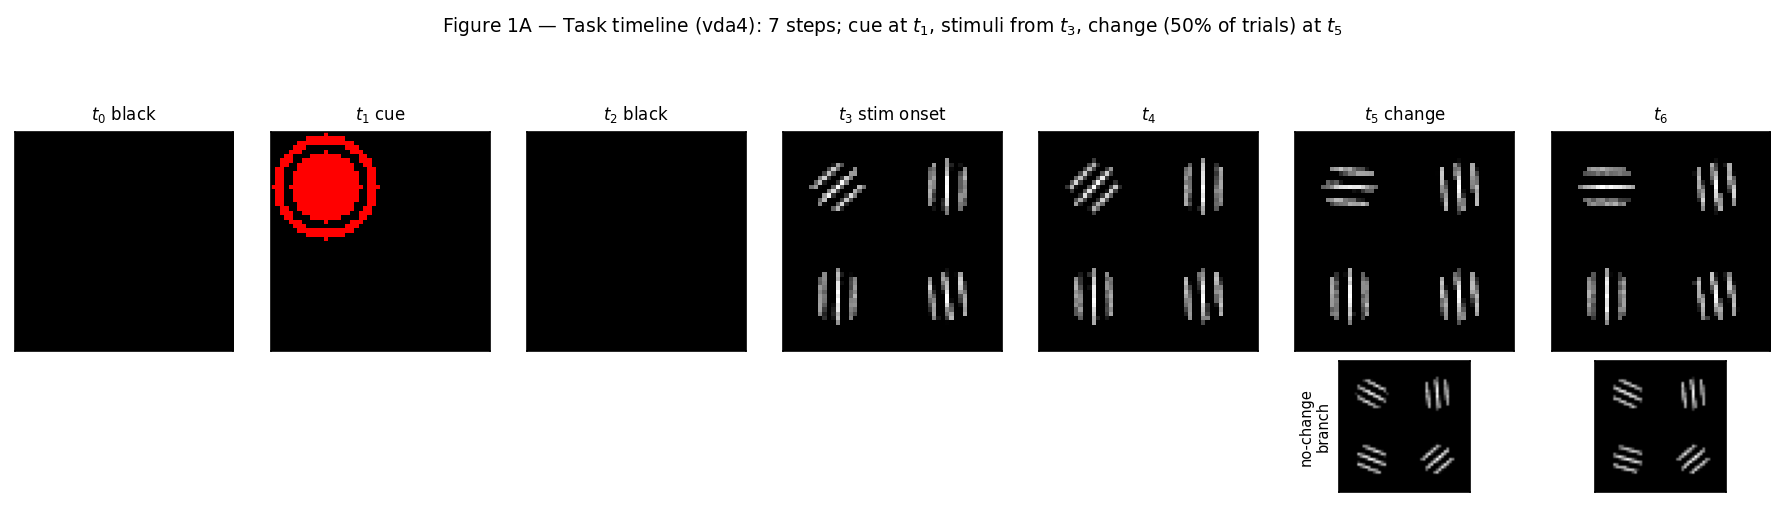
\includegraphics[width=\textwidth]{fig1A_task_timeline.png}\\[4pt]
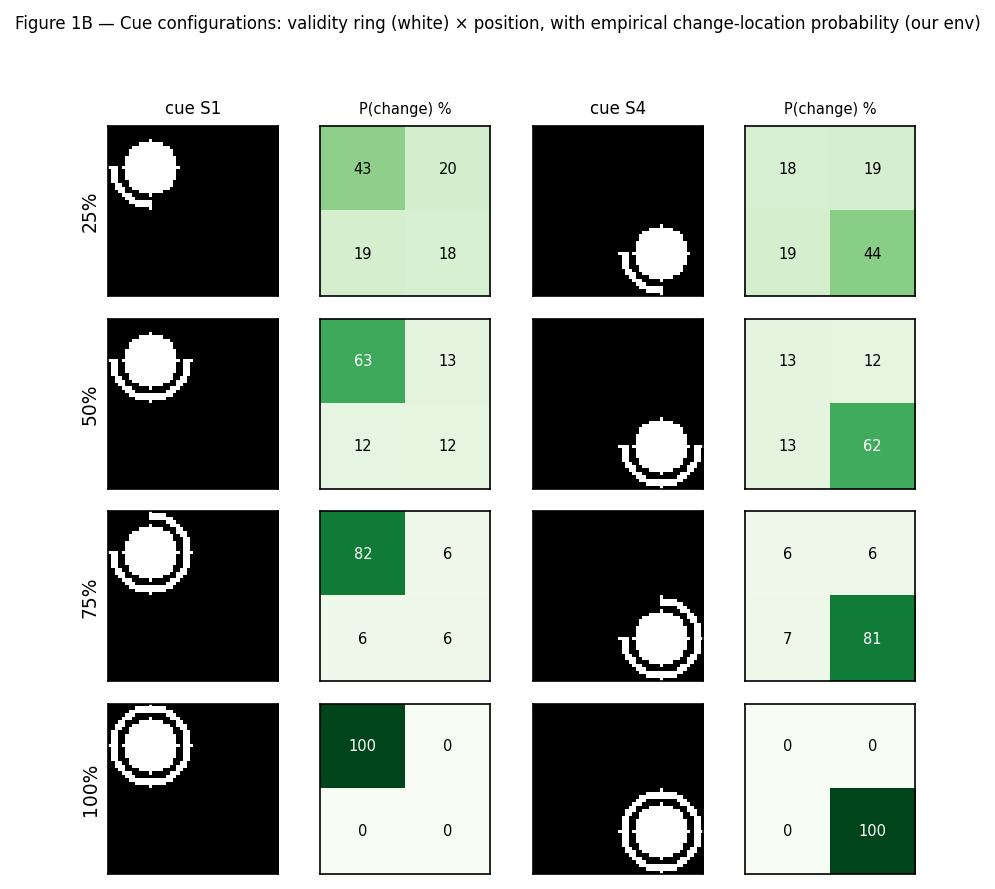
\includegraphics[width=0.6\textwidth]{fig1B_cue_configs.png}
\caption{\textbf{Fig 1 --- Task / environment.} Top: the 7-step trial timeline with the change /
no-change branch. Bottom: cue configurations (validity ring $\times$ position) with the empirical
change-location probability our environment produces.}\label{fig:task}\end{figure}

\begin{figure}[h]\centering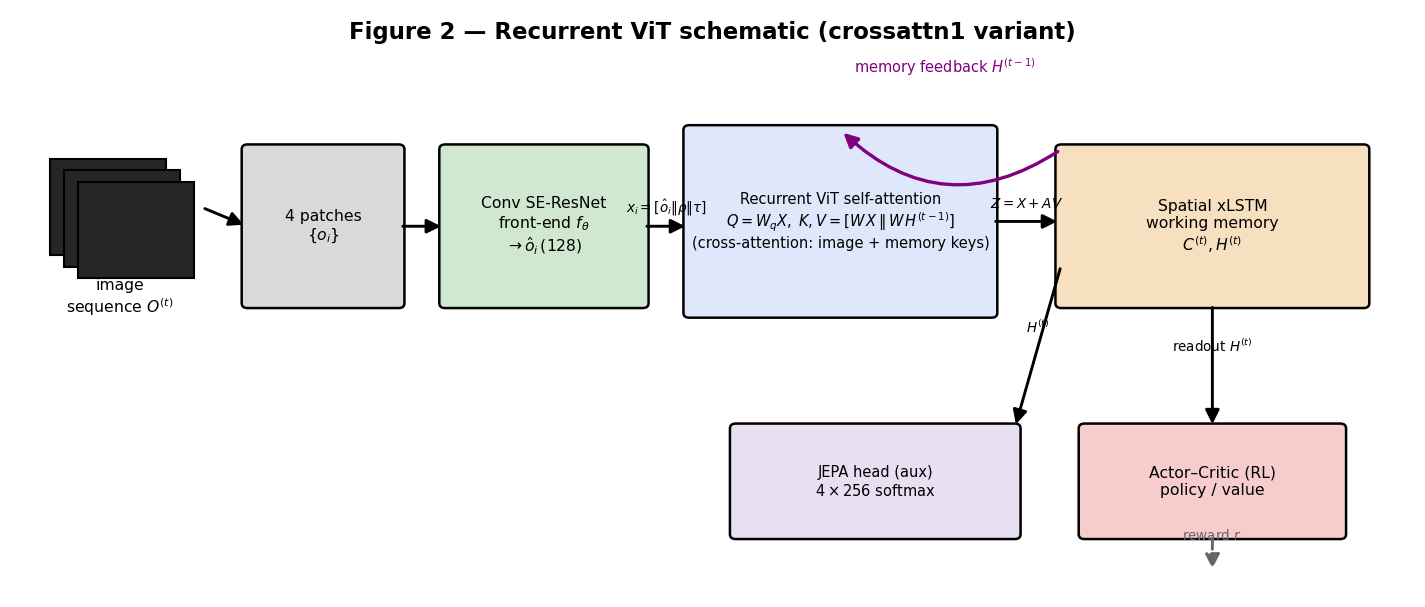
\includegraphics[width=\textwidth]{fig2_schematic_crossattn1.png}
\caption{\textbf{Fig 2 --- Model schematic (cross-attention variant).} Image sequence $\to$ four patches
$\to$ conv SE-ResNet front-end $\to$ recurrent-ViT self-attention with memory feedback ($K,V$ over
image$+$memory) $\to$ spatial xLSTM working memory $\to$ readout to actor--critic (RL) and a JEPA head.}
\label{fig:model}\end{figure}

\section{Behaviour: psychometrics and chronometrics}
The variant produces orderly sigmoidal psychometric and chronometric functions
(Fig.~\ref{fig:psy}) with the characteristic shapes of the original: response rate rises with $\Delta$,
floors near the false-alarm rate at $\Delta{=}0$, and saturates by $\sim\!30^\circ$; reaction time
decreases with $\Delta$. \emph{Divergence from the original:} the four validity conditions
($25/50/75/100\%$) are nearly superimposed, and the fitted logistic threshold (\emph{Position}) is flat
across validity ($13.8/13.8/13.9/14.0^\circ$). This variant therefore does \emph{not} reproduce the
original's validity-graded threshold shift---consistent with its perceiving the validity ring at the
cue frame but not retaining it. Fitted parameters are in Fig.~\ref{fig:psyp}.

\begin{figure}[h]\centering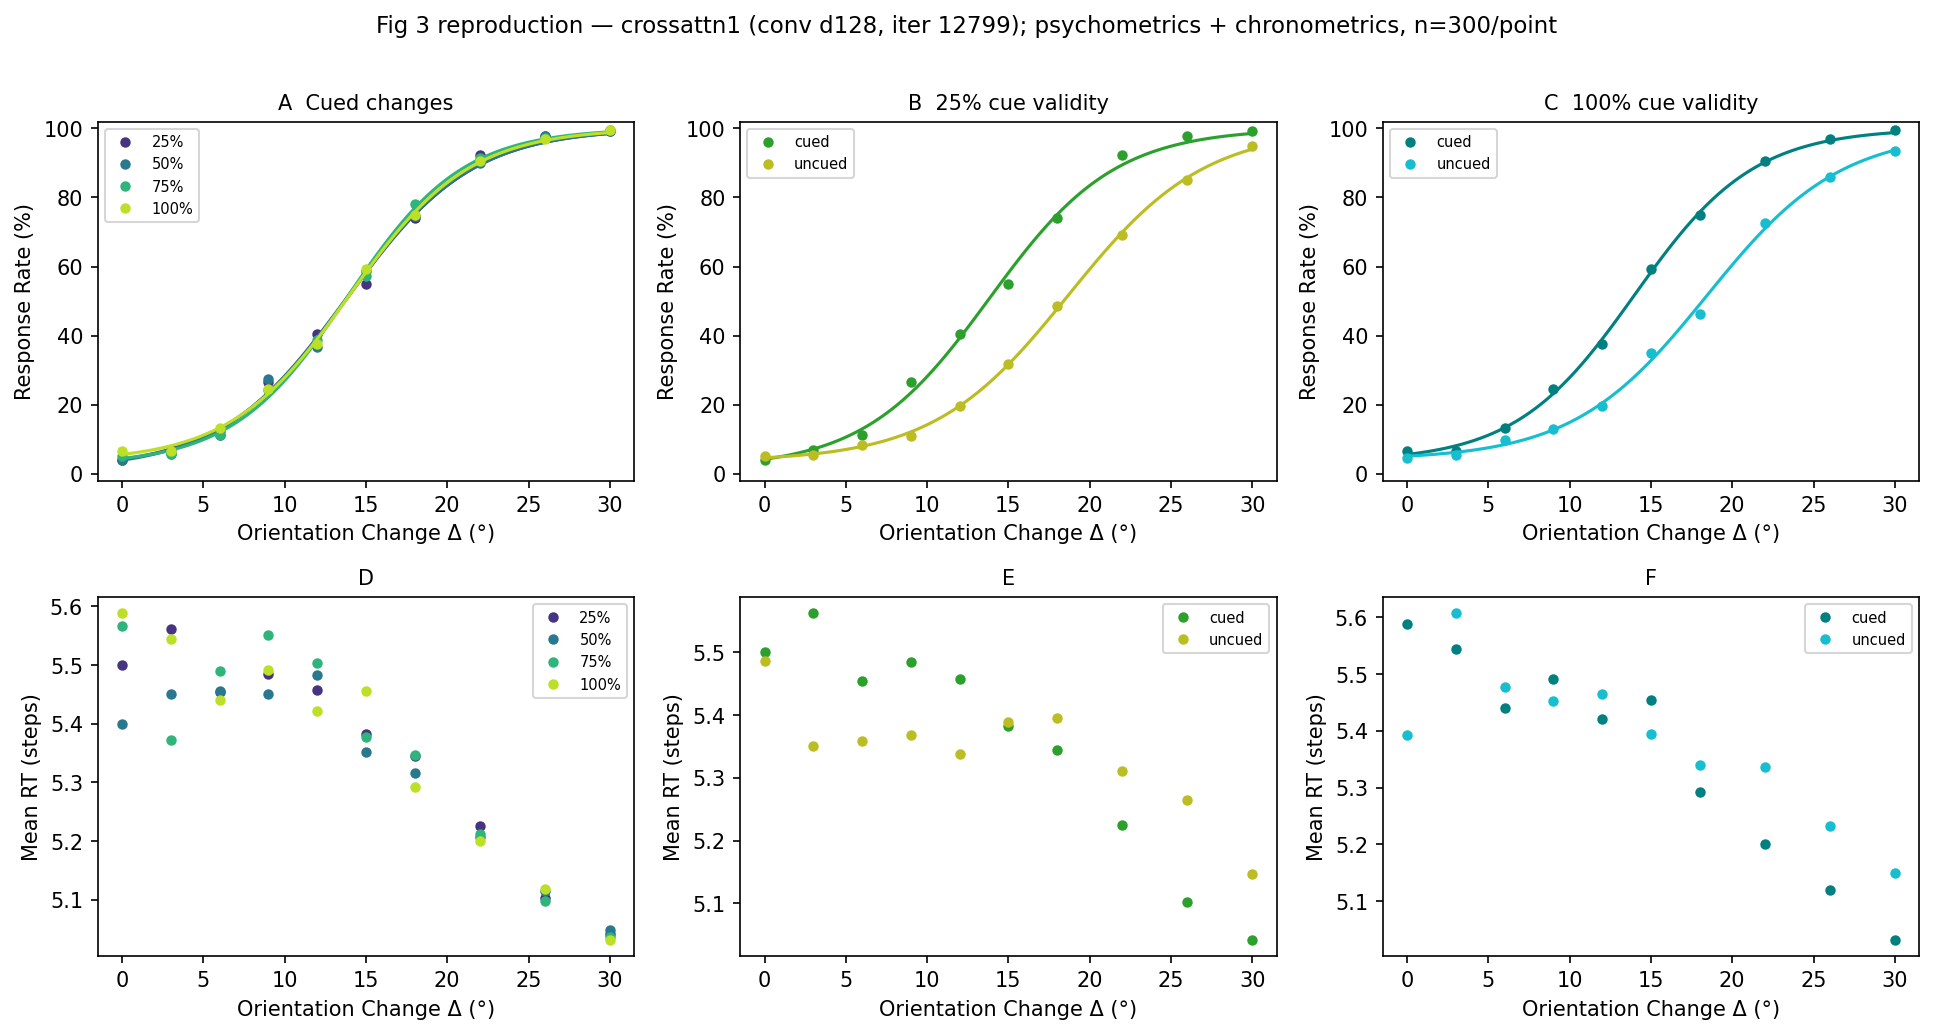
\includegraphics[width=\textwidth]{fig3_crossattn1.png}
\caption{\textbf{Fig 3 --- psychometrics and chronometrics.} A: response rate vs.\ $\Delta$ for cued
changes at four validities (superimposed for this variant). B, C: cued vs.\ uncued at $25\%$ and
$100\%$. D--F: mean reaction time. Points $n{=}300$; lines are 4-parameter logistic fits.}\label{fig:psy}\end{figure}
\begin{figure}[h]\centering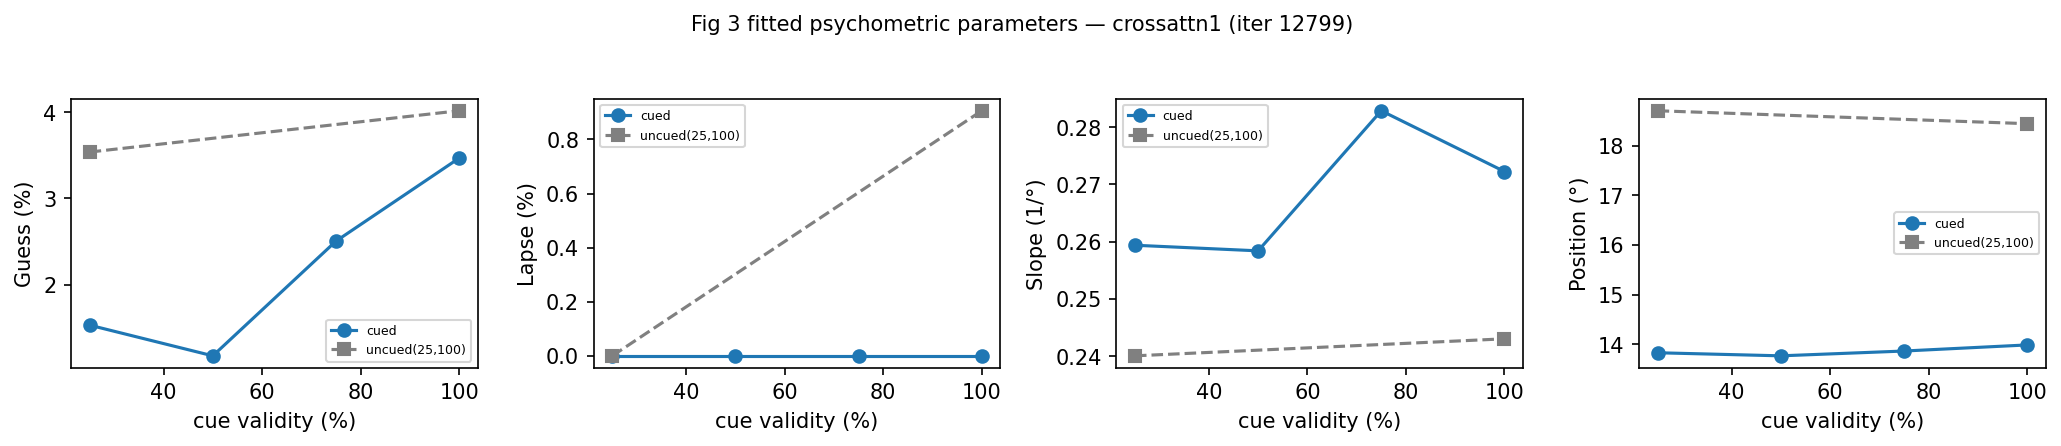
\includegraphics[width=0.95\textwidth]{fig3_crossattn1_params.png}
\caption{\textbf{Fitted psychometric parameters} (guess, lapse, slope, position) vs.\ cue validity, cued
and uncued.}\label{fig:psyp}\end{figure}

\section{Attention allocation dynamics}
Averaged recurrent self-attention (Fig.~\ref{fig:attn}) is flat at onset, becomes strongly biased
toward the cued location at the cue frame ($\alpha_1{\approx}0.73$ at $t{=}1$), and---because memory
sustains allocation without visual input---remains biased through the following blank. This anticipatory
maintenance of spatial priority in memory reproduces a core feature of the original. Panel B shows
$\alpha_1,\alpha_4$ across time; panel C shows $\alpha_1$ at the change frame vs.\ change magnitude at
the cued/uncued locations. Time-courses are again essentially \emph{invariant to displayed validity}.

\begin{figure}[h]\centering
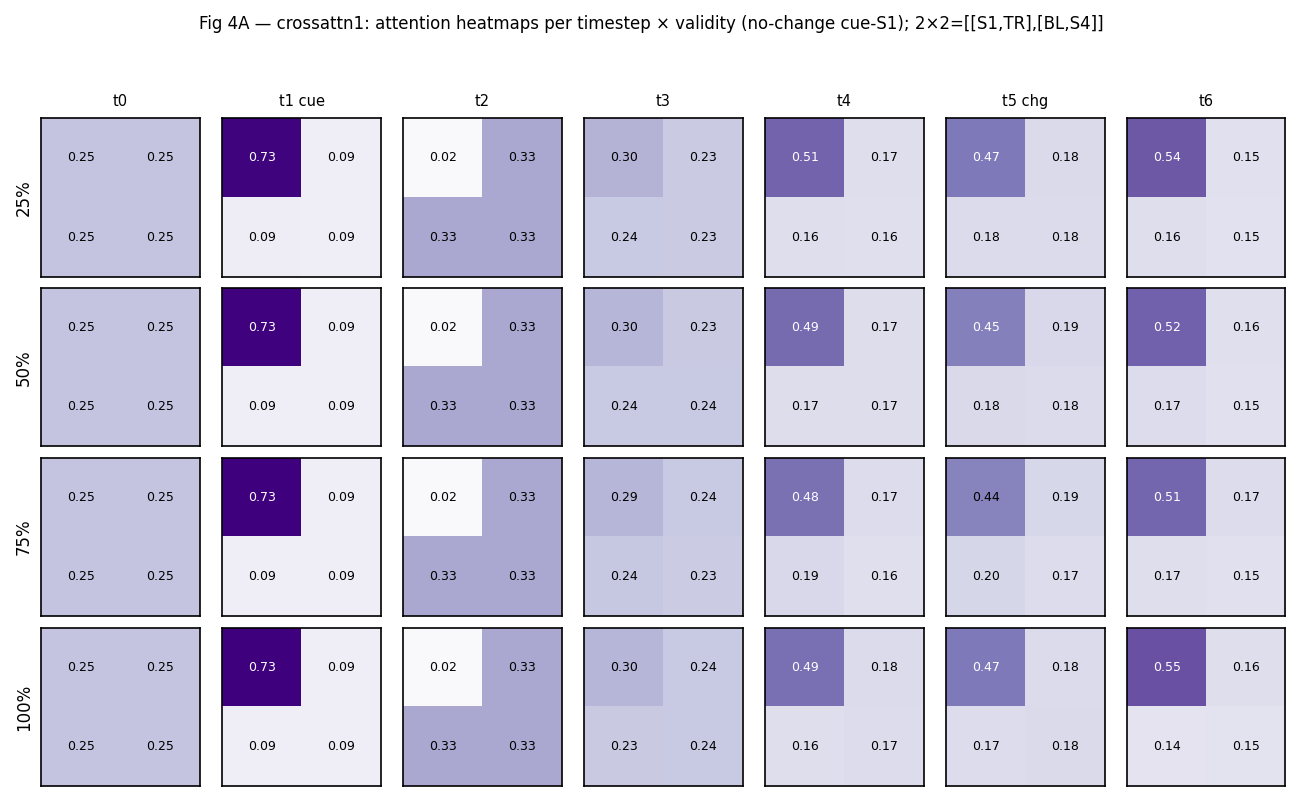
\includegraphics[width=\textwidth]{fig4A_crossattn1.png}\\[4pt]
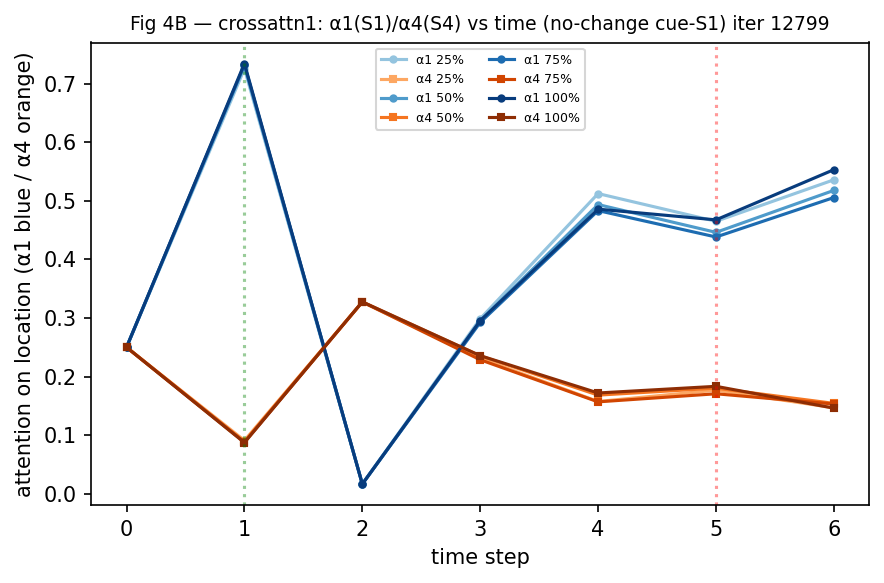
\includegraphics[width=0.47\textwidth]{fig4B_crossattn1.png}\hfill
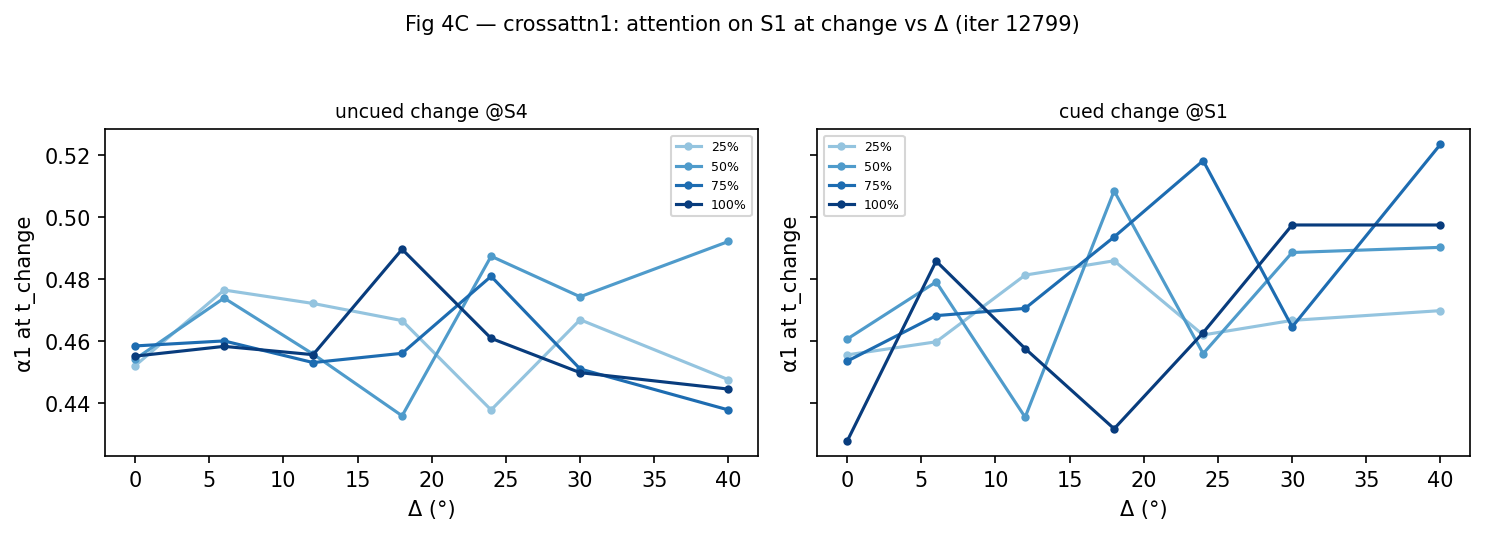
\includegraphics[width=0.47\textwidth]{fig4C_crossattn1.png}
\caption{\textbf{Fig 4 --- intrinsic attention dynamics.} Top: per-timestep attention heatmaps
($2\times2$) by validity on no-change cue-$S_1$ trials. Bottom left: $\alpha_1$/$\alpha_4$ vs.\ time.
Bottom right: $\alpha_1$ at the change frame vs.\ $\Delta$ at the uncued and cued locations.}\label{fig:attn}\end{figure}

\section{Feedback mechanism}
The original compares three memory$\to$vision feedback mechanisms (concatenation / additive /
multiplicative); our cross-attention variant instantiates the \emph{memory-as-tokens} (concatenation)
mechanism, in which the attention keys/values span image and memory tokens. Fig.~\ref{fig:fb} shows this
variant's feedback circuit alongside the four behavioural panels of the original's feedback figures:
cued response by validity (A), the behavioural effect of enhancing/suppressing attention on the cued
change (B), cued vs.\ uncued at $100\%$ (C), and the deployment of attention at the change frame (D).

\begin{figure}[h]\centering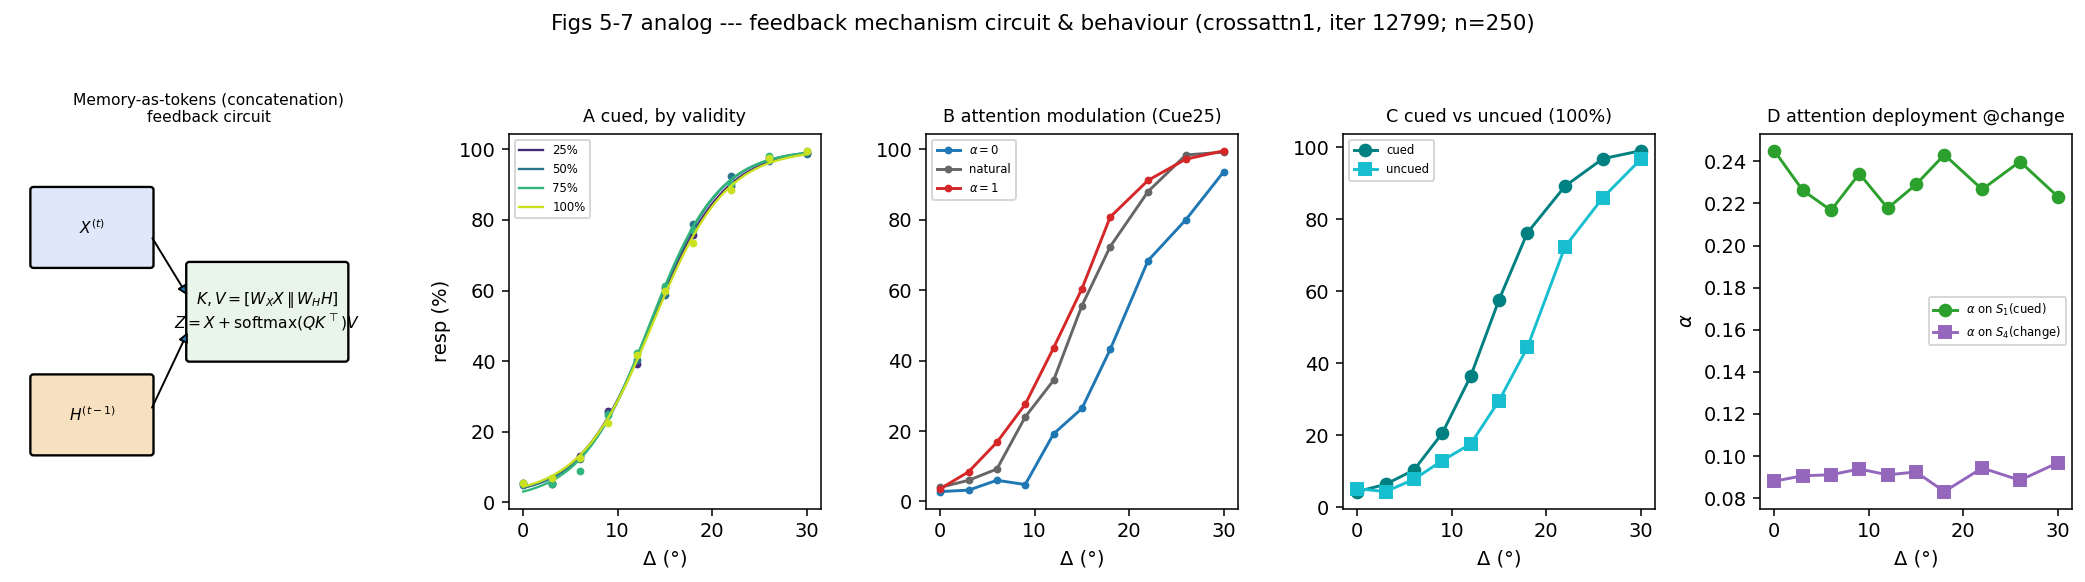
\includegraphics[width=\textwidth]{fig567_crossattn1.png}
\caption{\textbf{Figs 5--7 analog --- feedback mechanism circuit \& behaviour.} Left: the variant's
memory-as-tokens feedback circuit. A: cued response rate by validity. B: response under
enhanced/suppressed attention on the cued change. C: cued vs.\ uncued at $100\%$. D: attention deployed
on the cued ($S_1$) vs.\ change ($S_4$) location at the change frame vs.\ $\Delta$.}\label{fig:fb}\end{figure}

\section{Causal attention manipulations on behaviour}
Because the recurrent self-attention is interpretable, we causally perturb it by clamping the attention
allocated to a location at the change frame (Fig.~\ref{fig:manip}). Directing attention onto an
\emph{uncued} change ($\alpha_4{=}1$) raises detection (e.g.\ at $\Delta{=}18^\circ$, $0.67\to0.81$),
while \emph{suppressing} attention at the cued location ($\alpha_1{=}0$) \emph{also} raises it
($0.67\to0.75$)---the ``dual effect'' seen after unilateral superior-colliculus inactivation.
Parametrically shifting attention from cued to uncued grades the psychometric threshold (\emph{Position}
$13.8^\circ\!\to\!17.6^\circ$ as $\alpha_1$ falls $1.0\to0.1$; Fig.~\ref{fig:manipp}).

\begin{figure}[h]\centering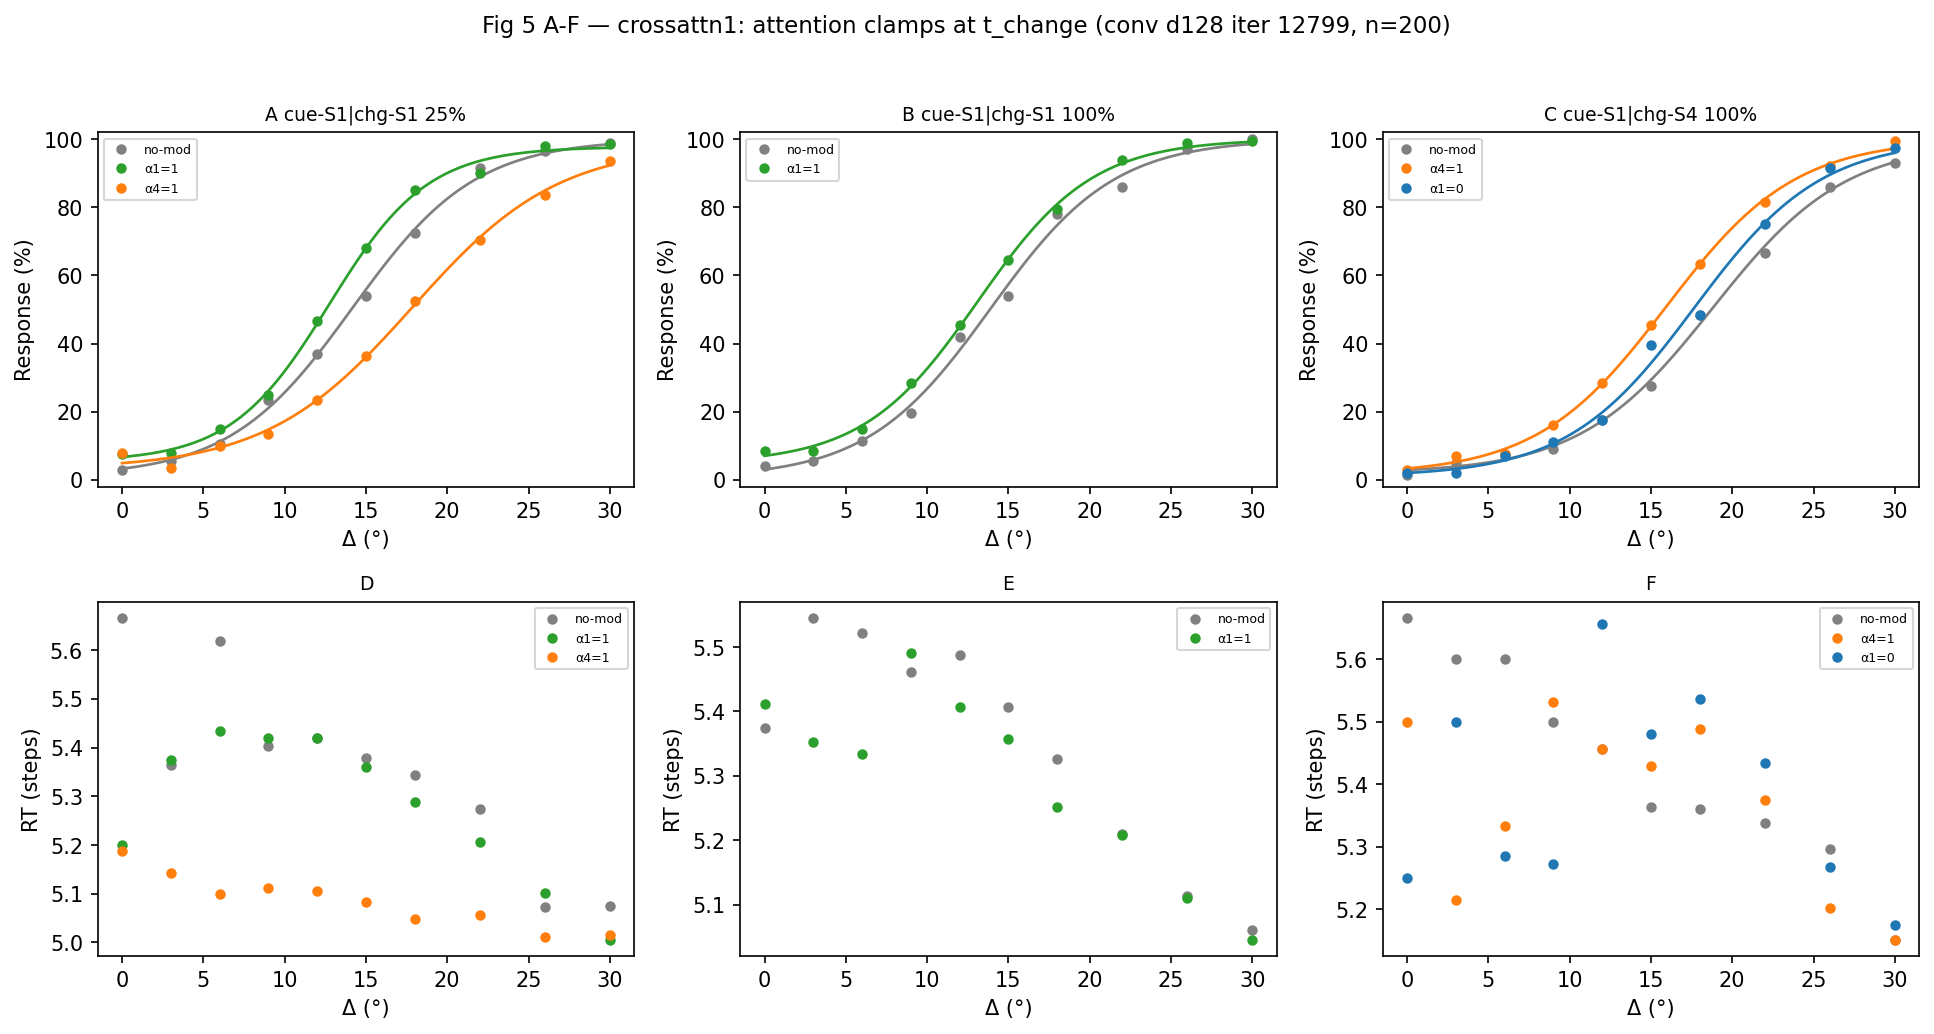
\includegraphics[width=\textwidth]{fig5AF_crossattn1.png}
\caption{\textbf{Attention clamps at $t_{\mathrm{change}}$.} Response rate (A--C) and reaction time
(D--F). C/F show the dual effect for an uncued change: both $\alpha_4{=}1$ and $\alpha_1{=}0$ improve
detection.}\label{fig:manip}\end{figure}
\begin{figure}[h]\centering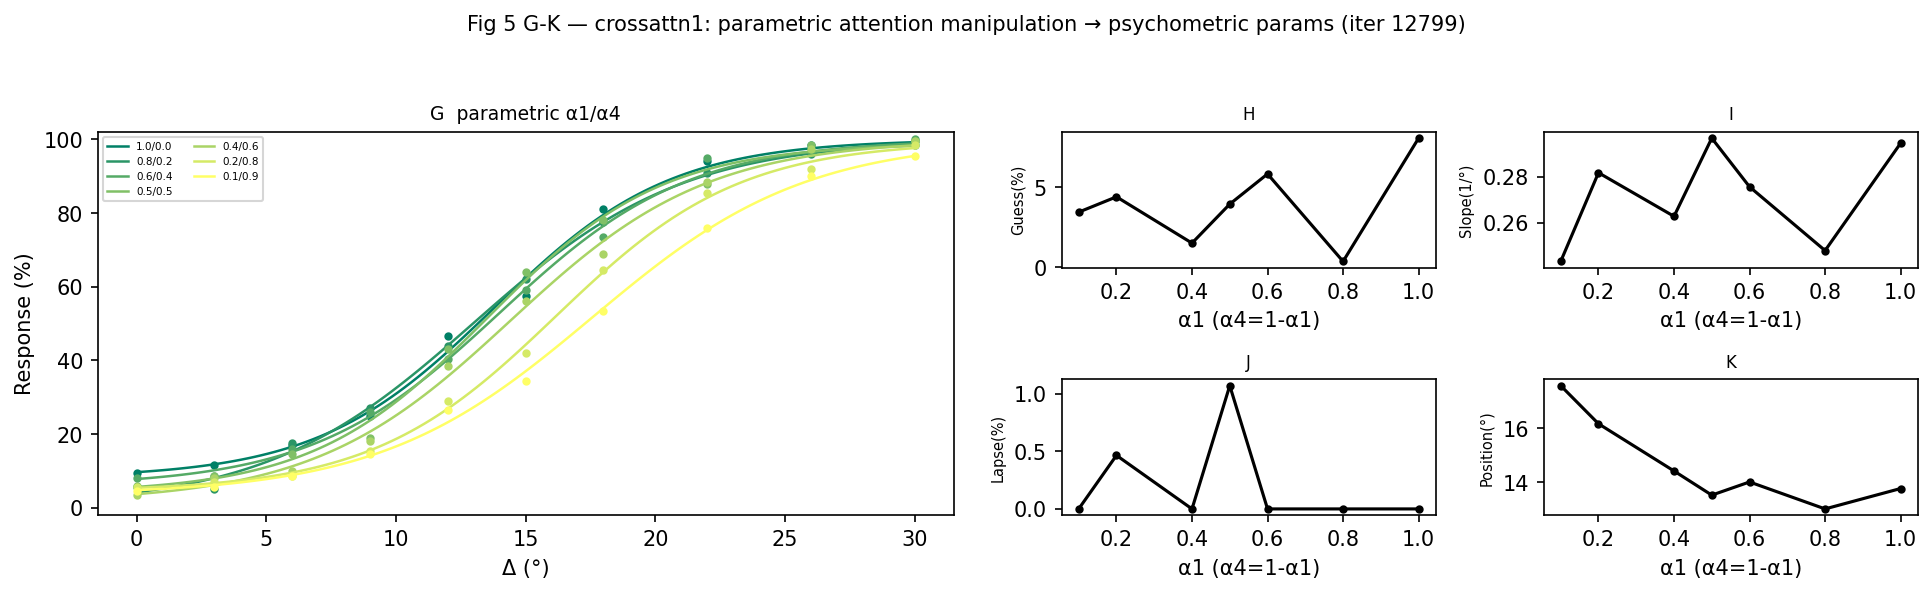
\includegraphics[width=\textwidth]{fig5GK_crossattn1.png}
\caption{\textbf{Parametric manipulation.} Shifting attention from uncued to cued grades the
psychometric function; fitted parameters show the effect falls mainly on threshold and lapse.}\label{fig:manipp}\end{figure}

\section{Decoding the mnemonic percept}
We train small feed-forward decoders (Linear--LayerNorm--ELU) on the recurrent states generated under
\emph{natural} (unmodulated) trials, then evaluate confusion matrices under attention modulation on
$S_1$. Change \emph{location} is decodable from the full mnemonic percept $H$
(Fig.~\ref{fig:dec8}), with decodability enhanced from $t{=}5$ to $t{=}6$ (temporal integration).
Enhancing attention on $S_1$ ($\alpha_1{=}1$) increases $S_1$ decodability while slightly reducing other
locations; suppressing it ($\alpha_1{=}0$) does the reverse. From a \emph{single} patch $h_1$, change
\emph{occurrence} is decodable above chance (Fig.~\ref{fig:dec9}), and forcing maximal attention on
$S_1$ suppresses the propagation of change signals into the $S_1$ slot---revealing that self-attention
is what \emph{amplifies} the change signal across memory slots. The actor's first activation layer
retains change \emph{occurrence} but loses spatial specificity (Fig.~\ref{fig:dec10}), and graded
inhibition of $\alpha_1$ produces a graded loss of $S_1$-change decodability (Fig.~\ref{fig:dec11}).

\begin{figure}[h]\centering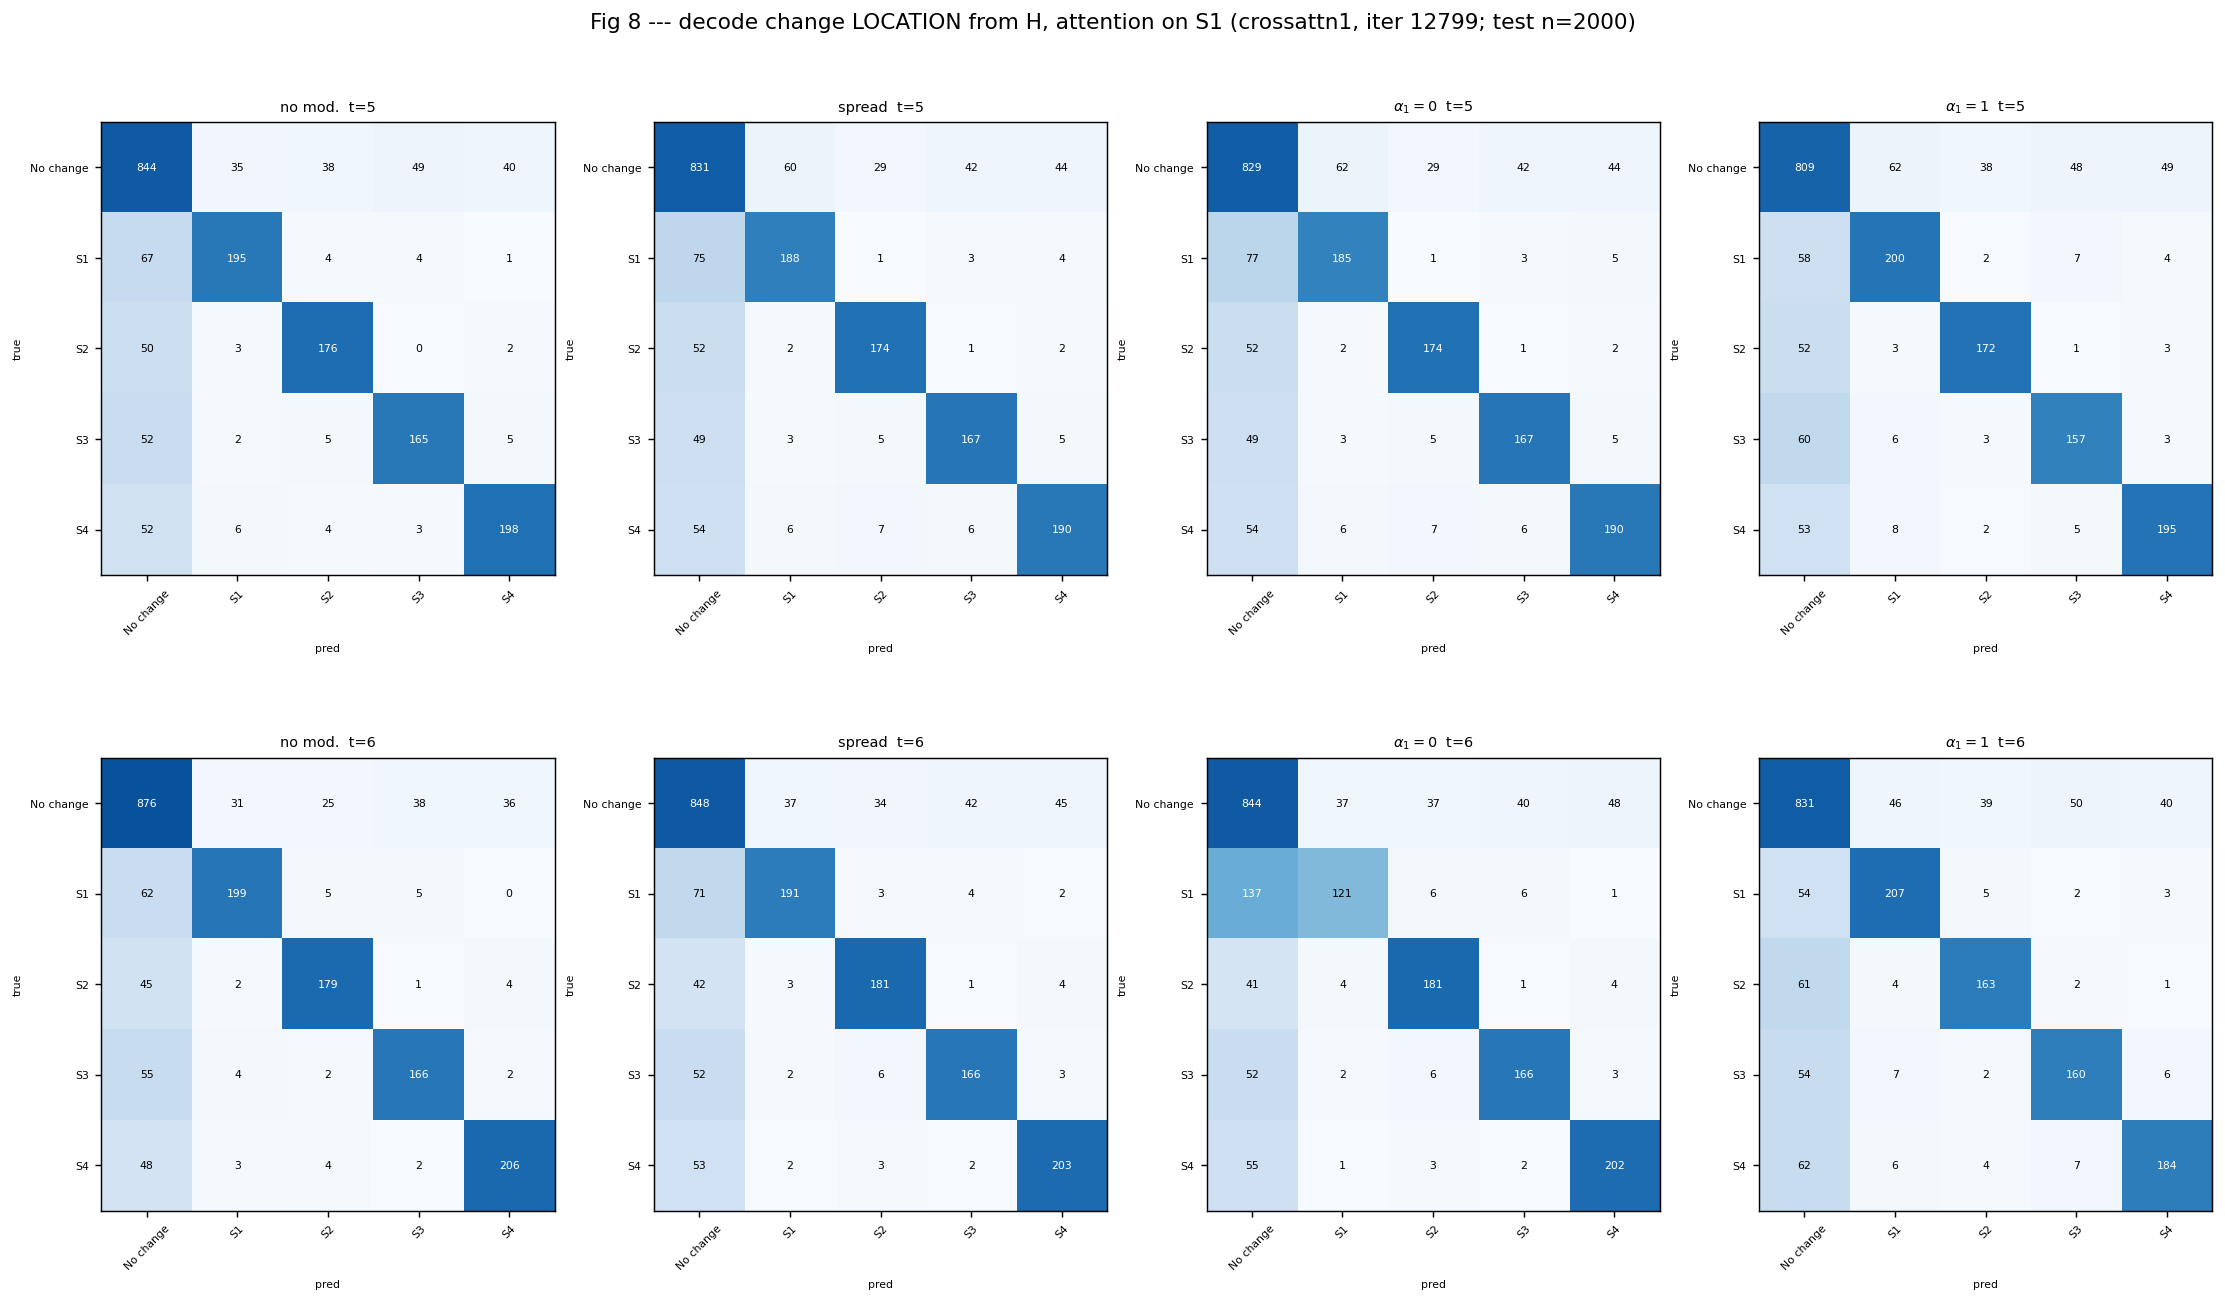
\includegraphics[width=\textwidth]{fig8_crossattn1.png}
\caption{\textbf{Fig 8 --- decode change LOCATION from $H$.} Confusion matrices (rows: $t{=}5$ top,
$t{=}6$ bottom) under \{no modulation, spread, $\alpha_1{=}0$, $\alpha_1{=}1$\}.}\label{fig:dec8}\end{figure}
\begin{figure}[h]\centering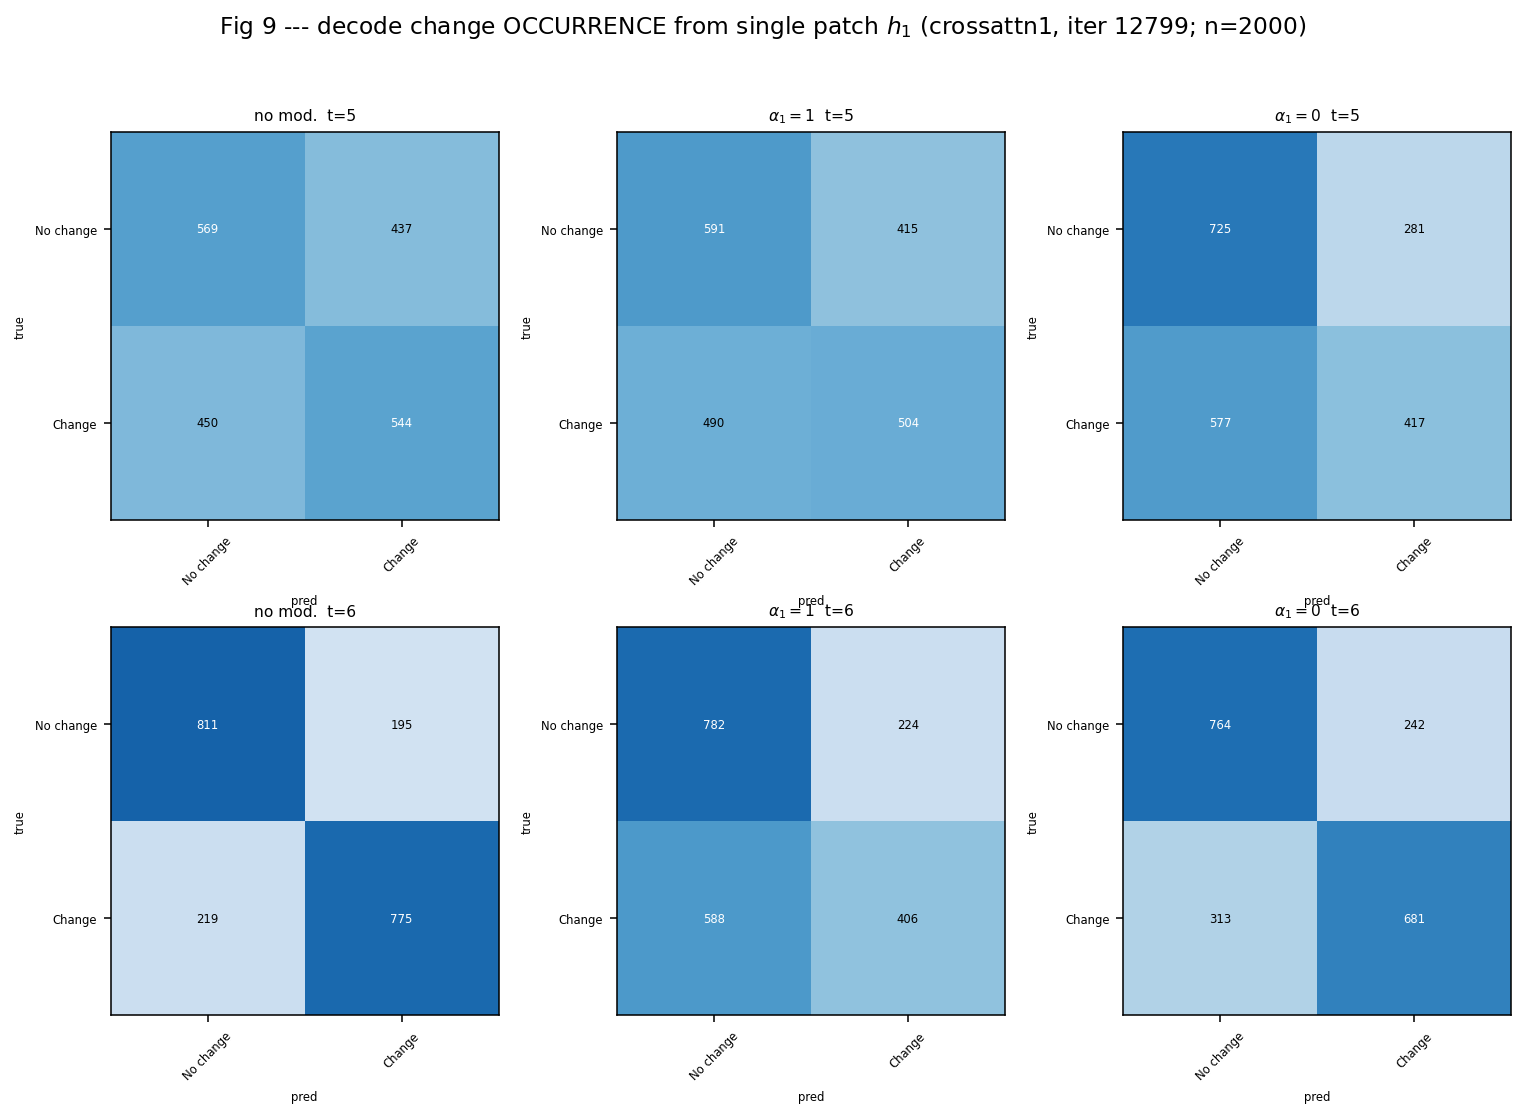
\includegraphics[width=0.85\textwidth]{fig9_crossattn1.png}
\caption{\textbf{Fig 9 --- decode change OCCURRENCE from single patch $h_1$}, $t{=}5$ (top) / $t{=}6$
(bottom), under \{no modulation, $\alpha_1{=}1$, $\alpha_1{=}0$\}.}\label{fig:dec9}\end{figure}
\begin{figure}[h]\centering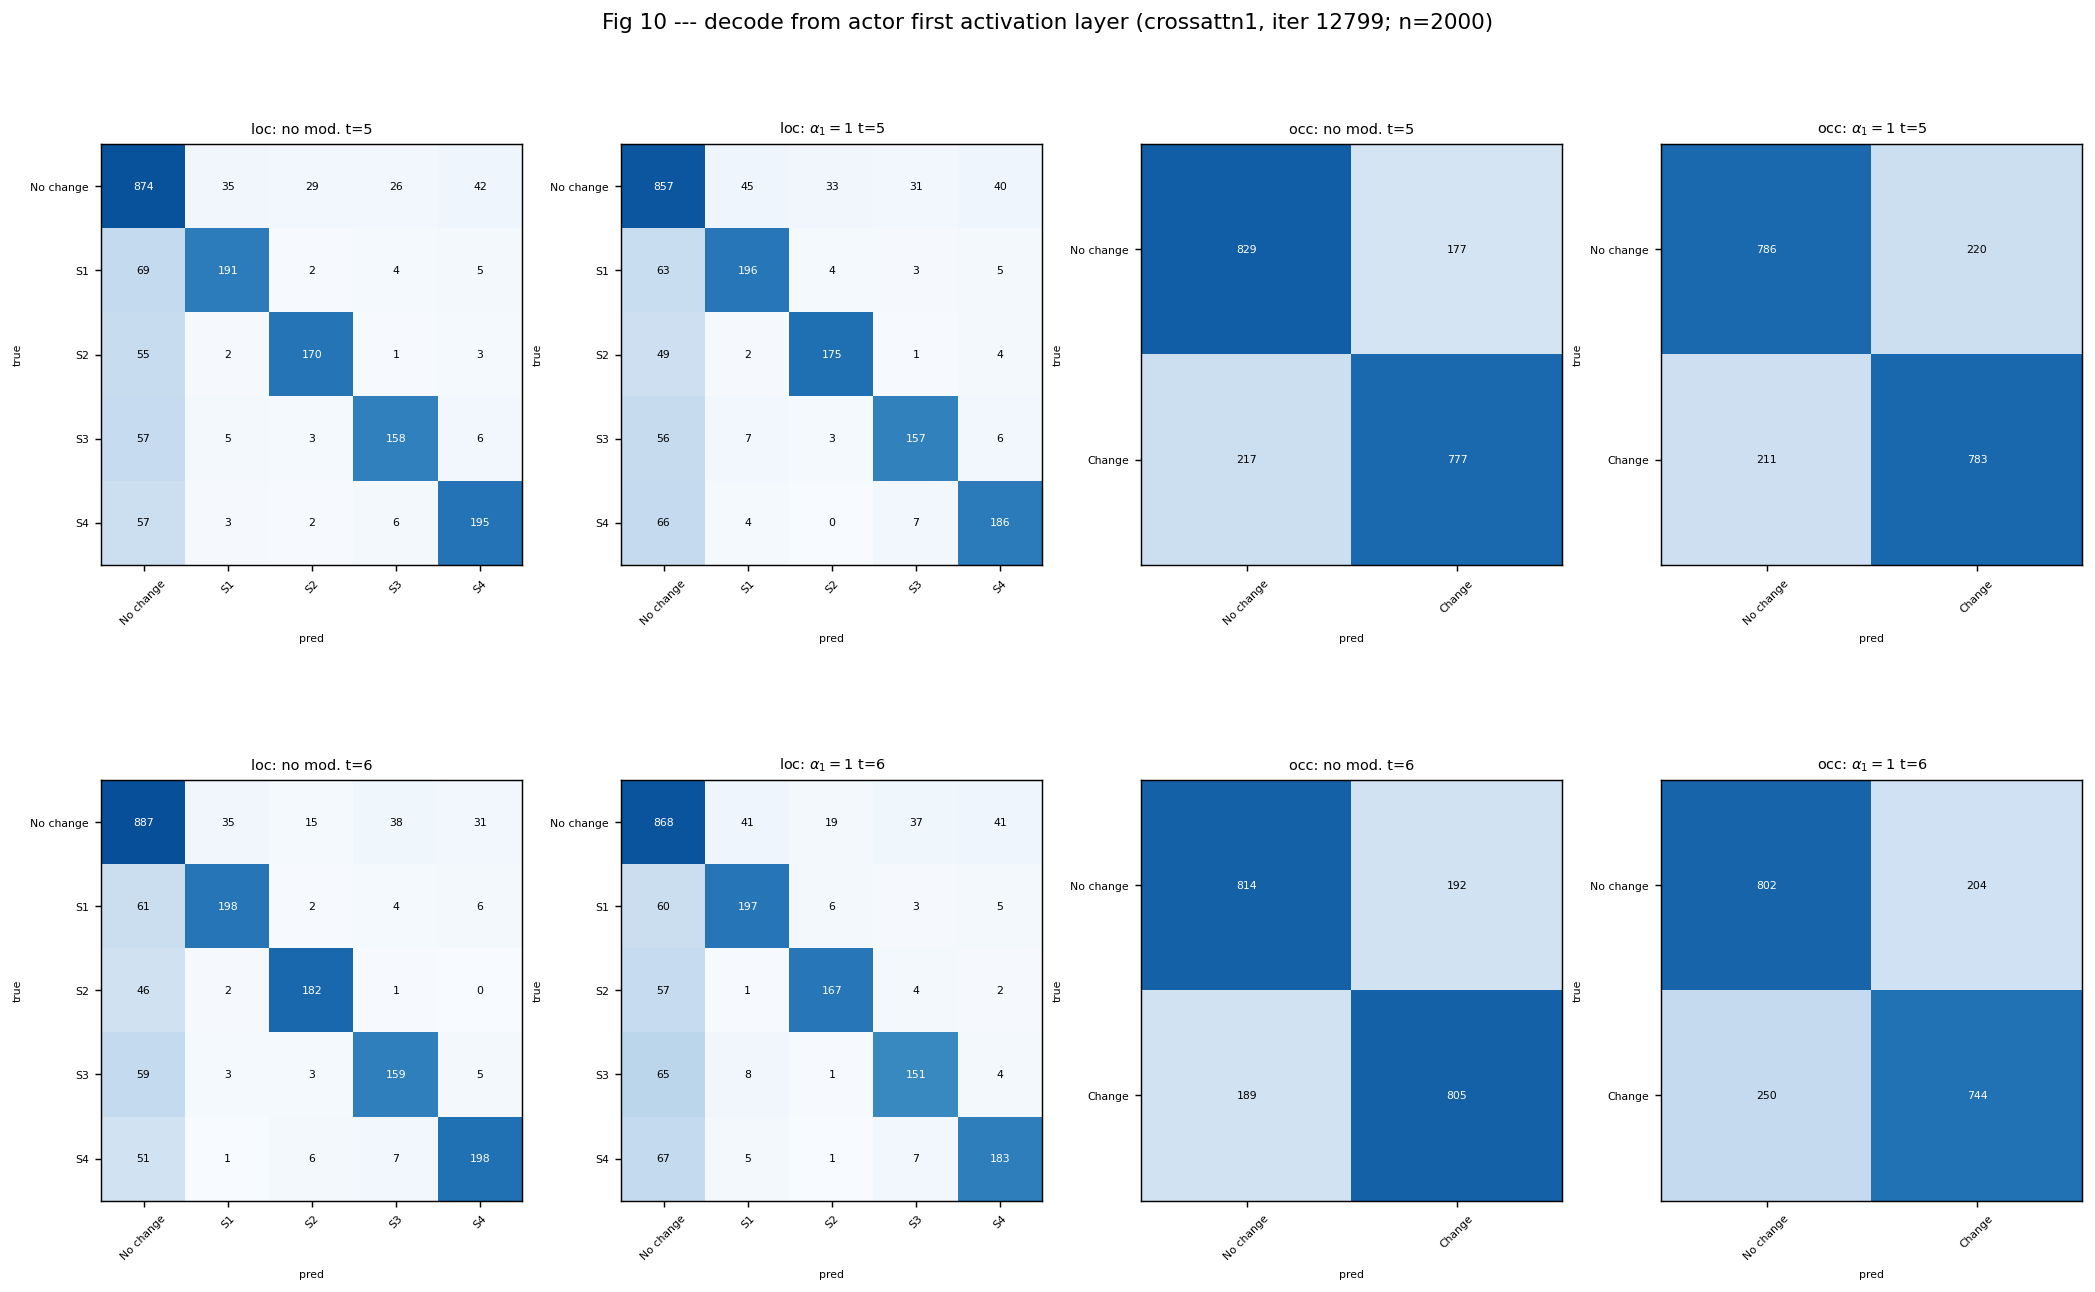
\includegraphics[width=\textwidth]{fig10_crossattn1.png}
\caption{\textbf{Fig 10 --- decode from the actor's first activation layer} (location, left; occurrence,
right), $t{=}5/6$, natural vs.\ $\alpha_1{=}1$.}\label{fig:dec10}\end{figure}
\begin{figure}[h]\centering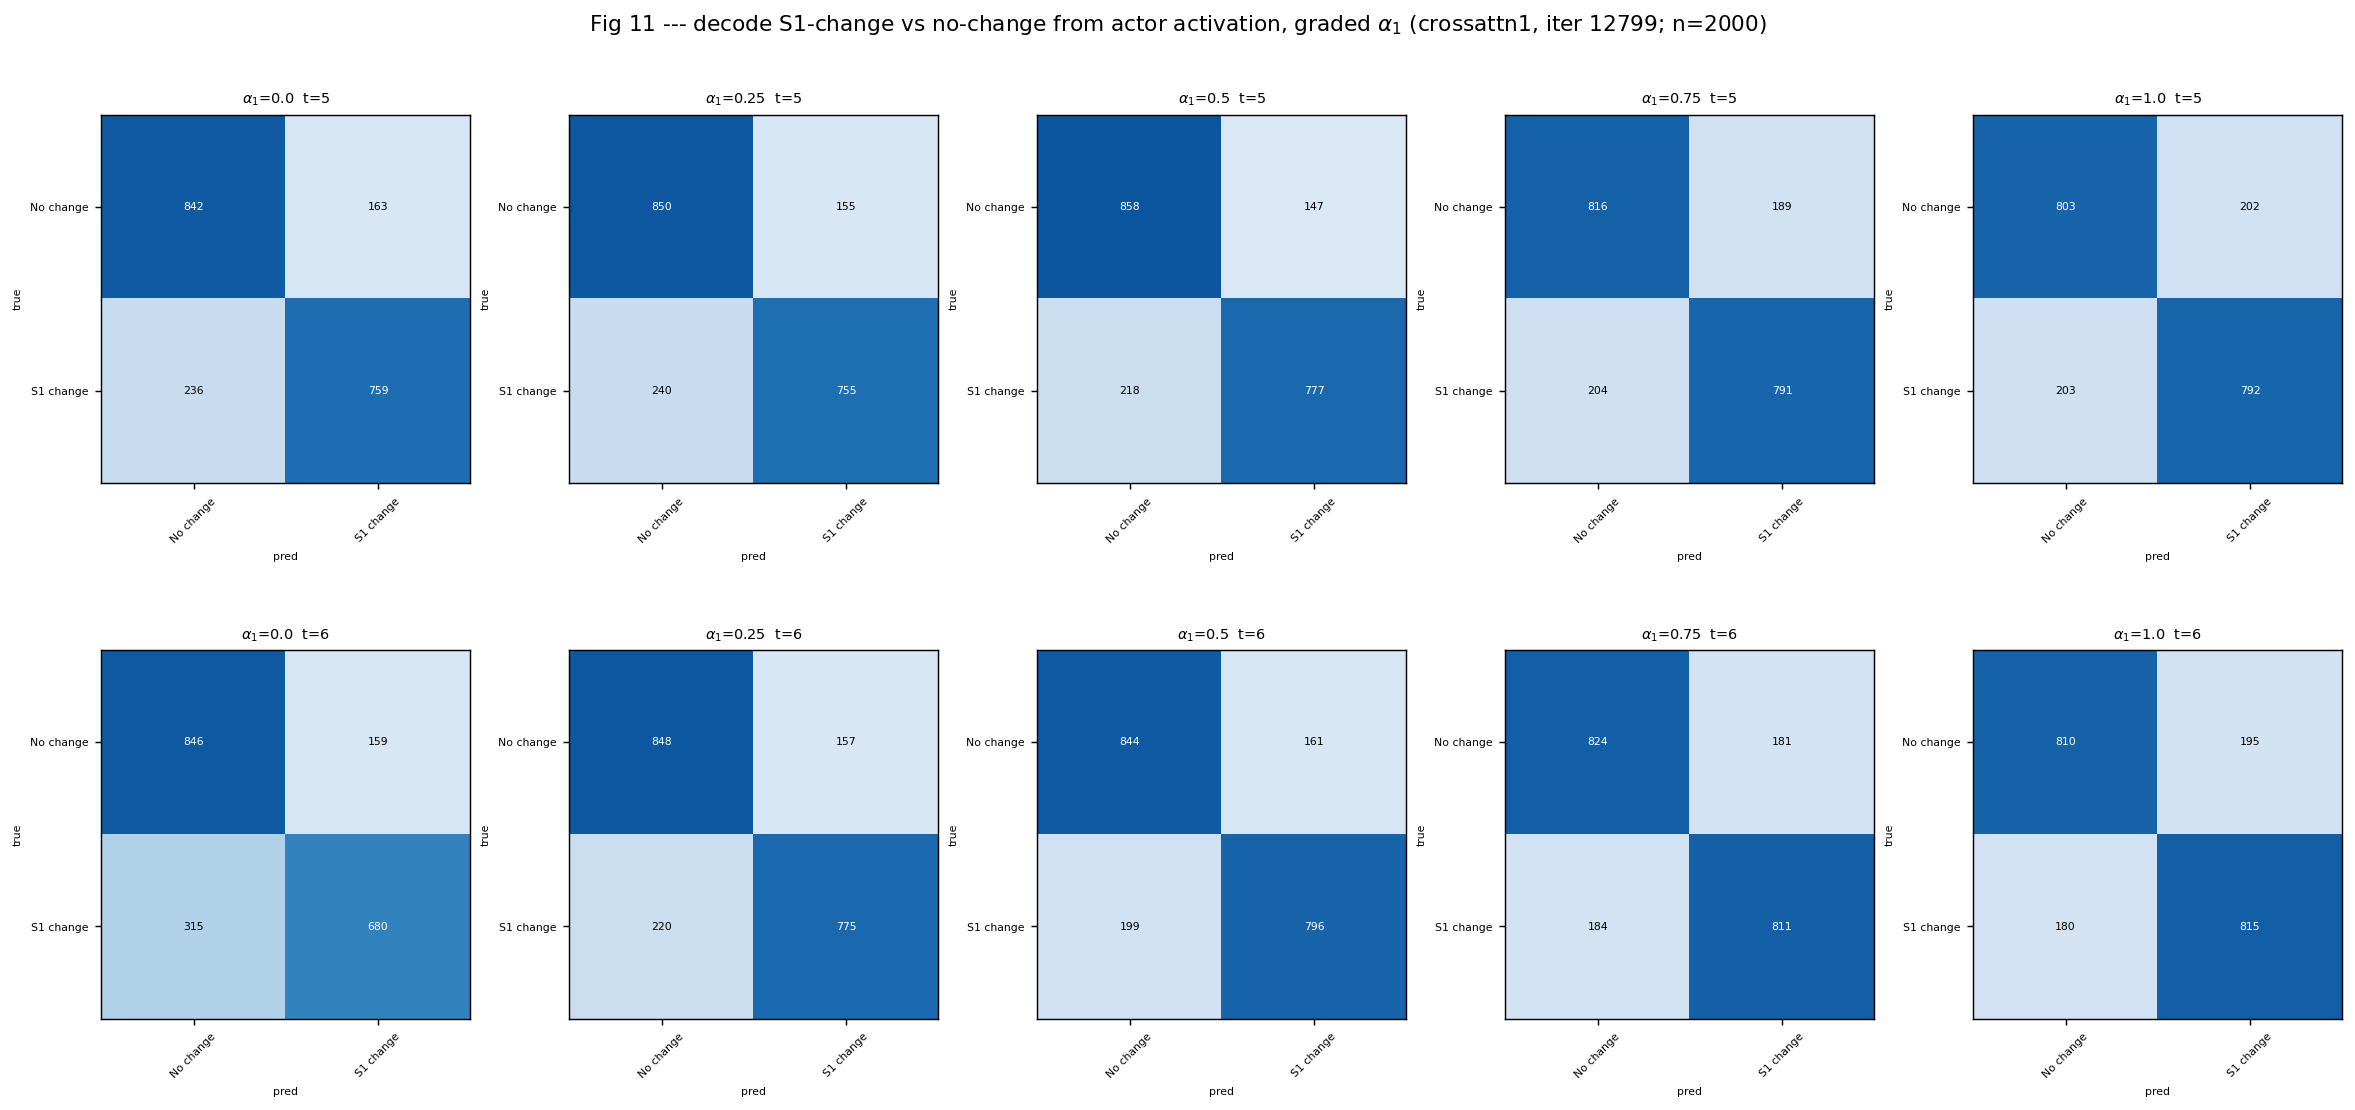
\includegraphics[width=\textwidth]{fig11_crossattn1.png}
\caption{\textbf{Fig 11 --- decode $S_1$-change vs.\ no-change from the actor activation} under graded
$\alpha_1$ inhibition ($0\to1$), $t{=}5$ (top) / $t{=}6$ (bottom).}\label{fig:dec11}\end{figure}

\section{Actor-logit geometry}
The final actor logits at the change frame lie on a competitive, anti-correlated Declare-Change vs.\
Wait axis, graded by change magnitude and largely independent of change location
(Fig.~\ref{fig:log12}). Attentional modulation shifts the distribution along this axis: enhancing
$\alpha_1$ pushes mass toward Declare-Change for $S_1$ changes, and suppressing it withdraws mass toward
Wait (Fig.~\ref{fig:log13}).

\begin{figure}[h]\centering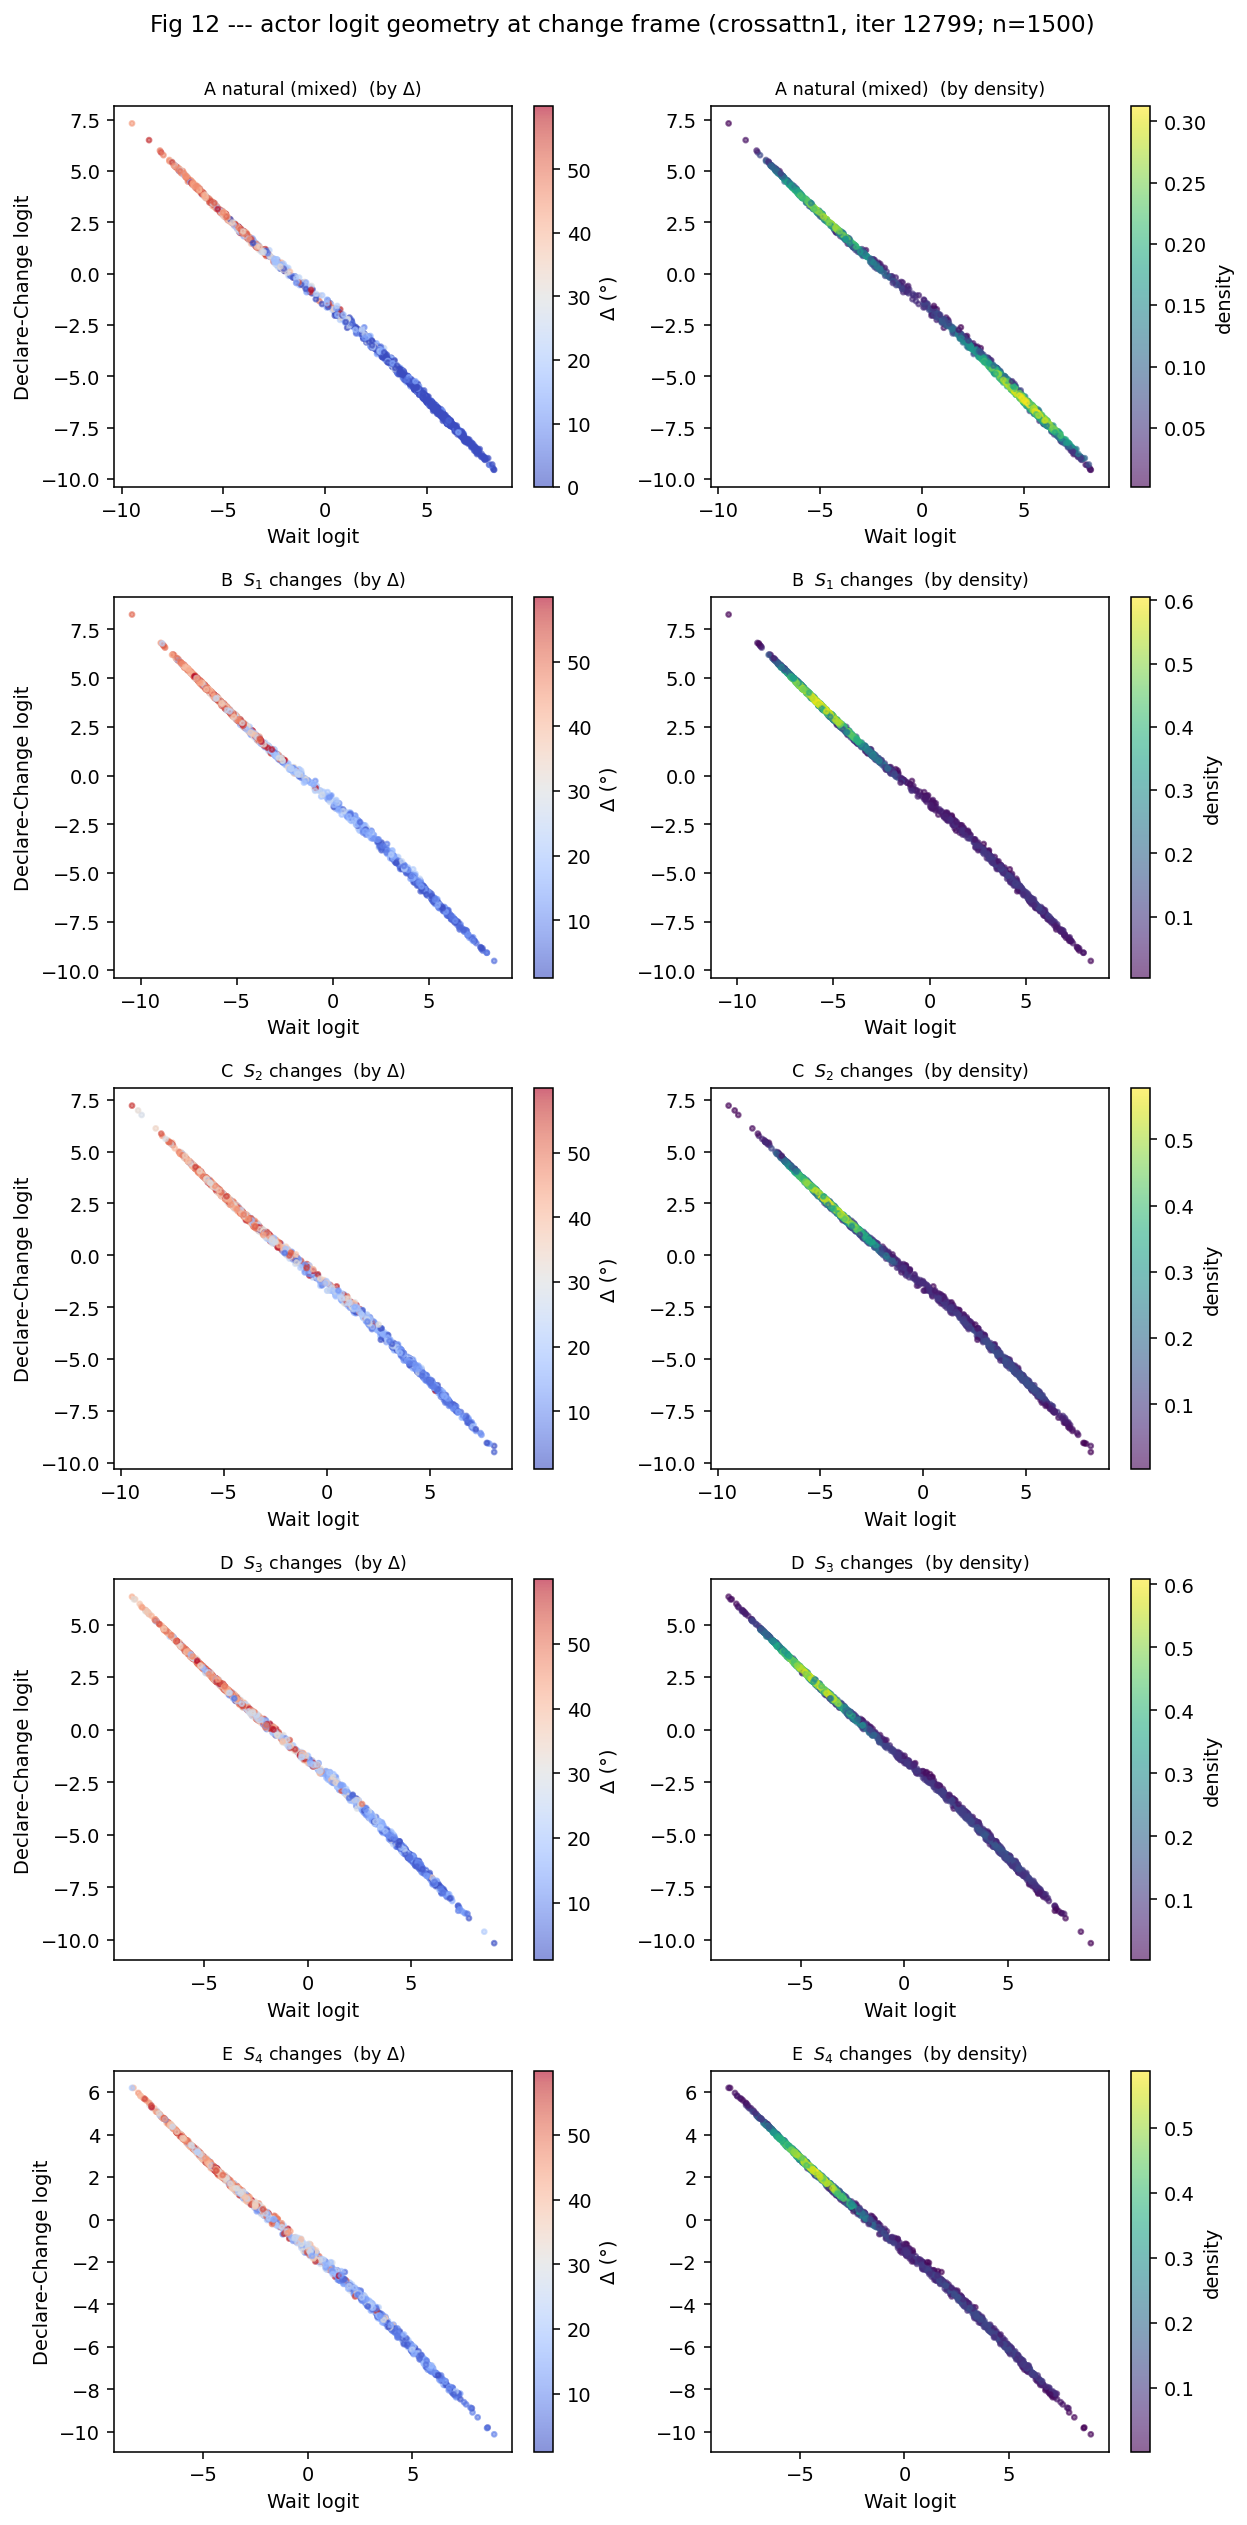
\includegraphics[width=0.62\textwidth]{fig12_crossattn1.png}
\caption{\textbf{Fig 12 --- actor logit geometry} at the change frame. A: natural mixed trials. B--E:
changes constrained to $S_1$--$S_4$. Left of each: coloured by $\Delta$; right: by 2D density.}\label{fig:log12}\end{figure}
\begin{figure}[h]\centering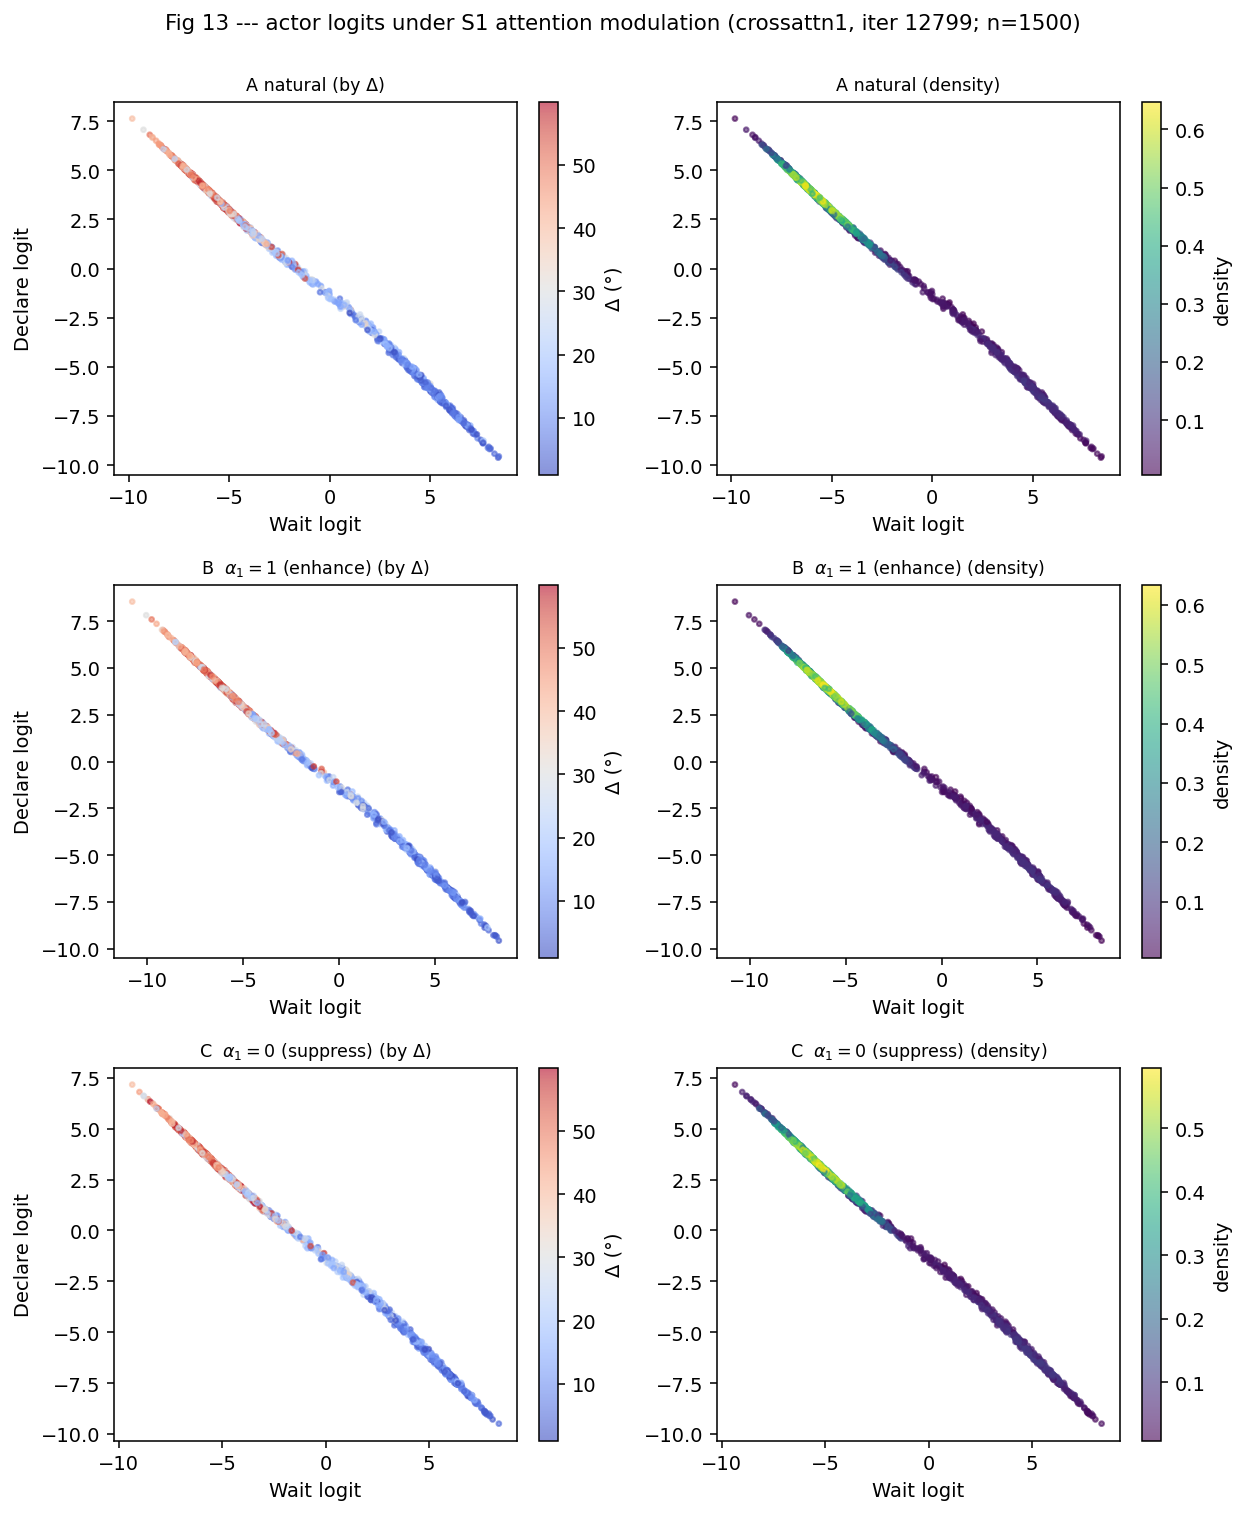
\includegraphics[width=0.62\textwidth]{fig13_crossattn1.png}
\caption{\textbf{Fig 13 --- actor logits under $S_1$ attention modulation.} A natural, B $\alpha_1{=}1$,
C $\alpha_1{=}0$; coloured by $\Delta$ (left) and density (right).}\label{fig:log13}\end{figure}

\section{Value, TD error and entropy}
From the distributional critic we read the scalar value $V(t)$; under the forced-wait rollout the
value-based TD surprise at the change, $\delta{=}\gamma V_6{-}V_5$, isolates the value jump at change
onset. The value $V$ grows monotonically with change magnitude and is higher for cued than uncued changes
(Fig.~\ref{fig:td14}B), while the value-based TD surprise stays positive---a value jump at change
onset---and is largest at the extremes (Fig.~\ref{fig:td14}A); enhancing attention on an uncued change
raises both the TD surprise and the hit rate ($30\%\!\to\!66\%$; Fig.~\ref{fig:td14}C,D). Policy entropy
is low throughout---the greedy actor is confident---and only weakly modulated by attention; the clearer
signature is the criterion--value coupling: as attention on $S_1$ is enhanced the value rises
($V\!:3.93\to4.11$) and the criterion falls in step ($c\!:1.05\to0.31$; Fig.~\ref{fig:ent15}).

\begin{figure}[h]\centering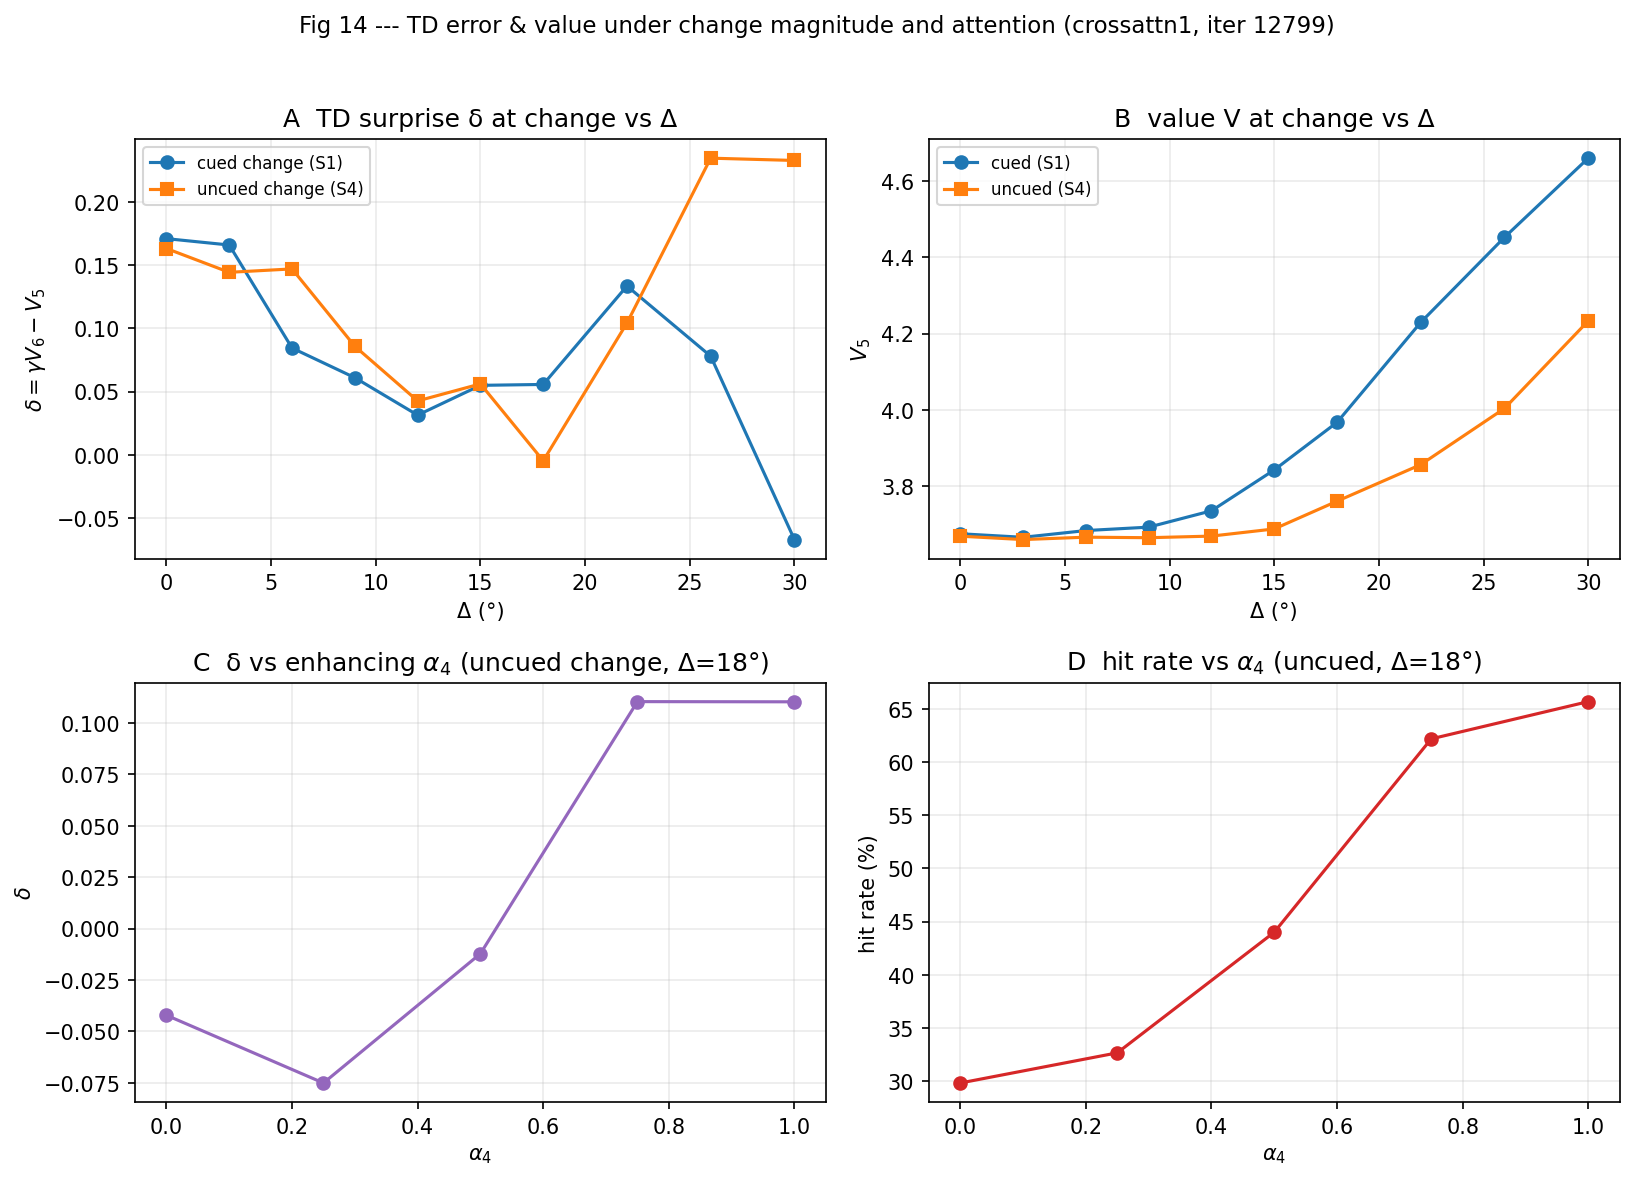
\includegraphics[width=\textwidth]{fig14_crossattn1.png}
\caption{\textbf{Fig 14 --- TD error \& value.} A: $\delta$ at change vs.\ $\Delta$, cued vs.\ uncued.
B: $V$ at change vs.\ $\Delta$. C: $\delta$ vs.\ enhancing $\alpha_4$ (uncued change). D: hit rate vs.\
$\alpha_4$.}\label{fig:td14}\end{figure}
\begin{figure}[h]\centering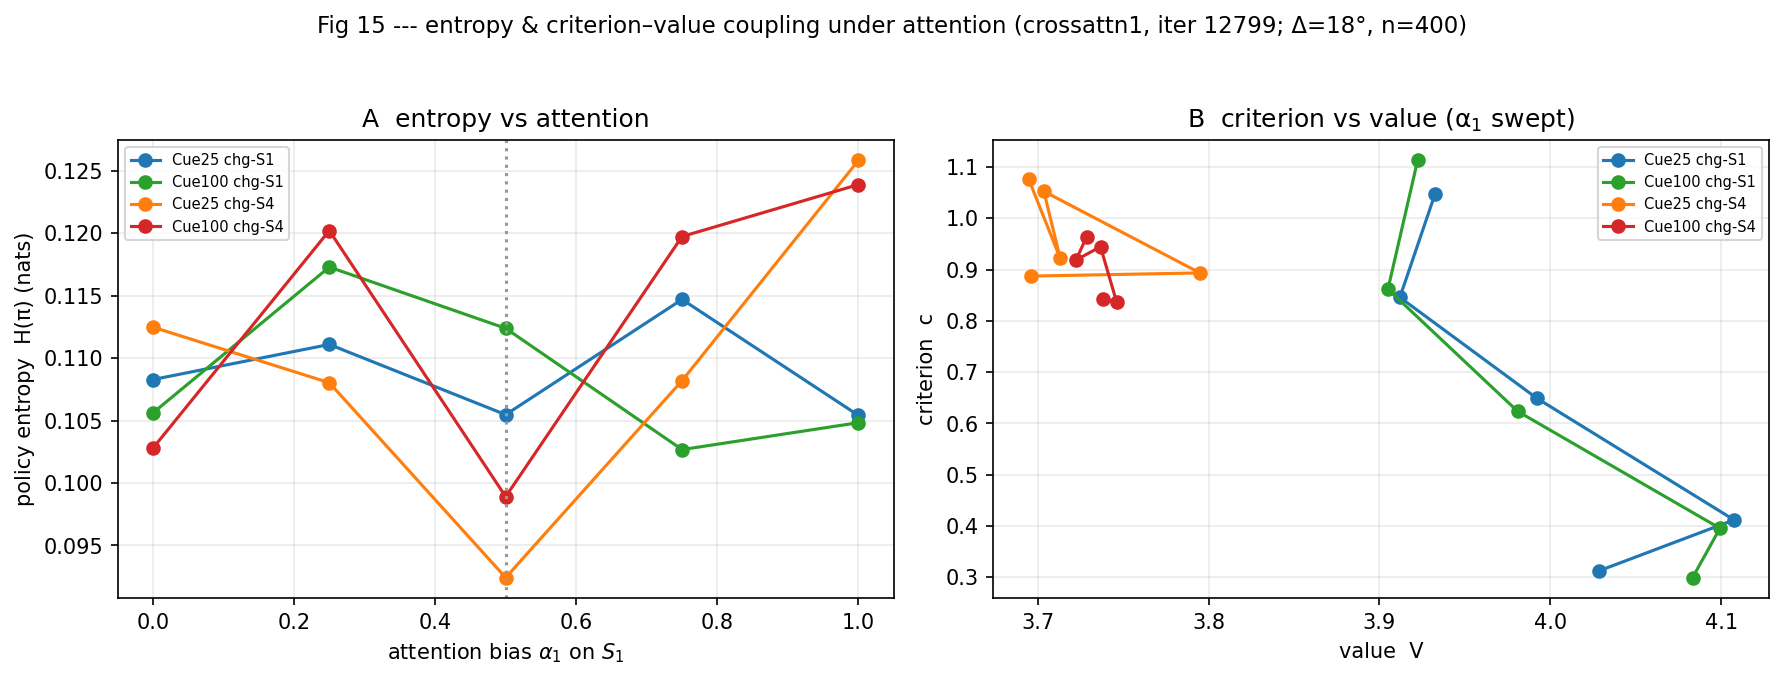
\includegraphics[width=0.95\textwidth]{fig15_crossattn1.png}
\caption{\textbf{Fig 15 --- entropy \& criterion--value coupling.} A: policy entropy at change vs.\
graded $\alpha_1$, four conditions. B: criterion $c$ vs.\ value $V$ as $\alpha_1$ is swept.}\label{fig:ent15}\end{figure}

\section{Signal detection: criterion \& sensitivity (``stimulation'' experiments)}
Treating a declared change as a ``yes'' response, we compute the signal-detection criterion
$c{=}-\tfrac12\!\big(z(\theta_H){+}z(\theta_{FA})\big)$ and sensitivity $d'{=}z(\theta_H){-}z(\theta_{FA})$
as attention on $S_1$ is biased parametrically, applied at cue-time ($t{=}1$) or change-time ($t{=}5$)
(Fig.~\ref{fig:sdt16}). Two clean signatures emerge, paralleling attentional microstimulation studies:
(i) enhancing attention on the change location lowers the \emph{criterion} (a more liberal ``change''
bias), and (ii) directing attention \emph{toward} the true change preserves/raises \emph{sensitivity}
whereas directing it \emph{away} (biasing $S_1$ when the change is at $S_4$) markedly reduces $d'$. Thus
even though the variant ignores displayed validity, its attention is causally load-bearing for the
decision variable in exactly the SDT terms of the original.

\begin{figure}[h]\centering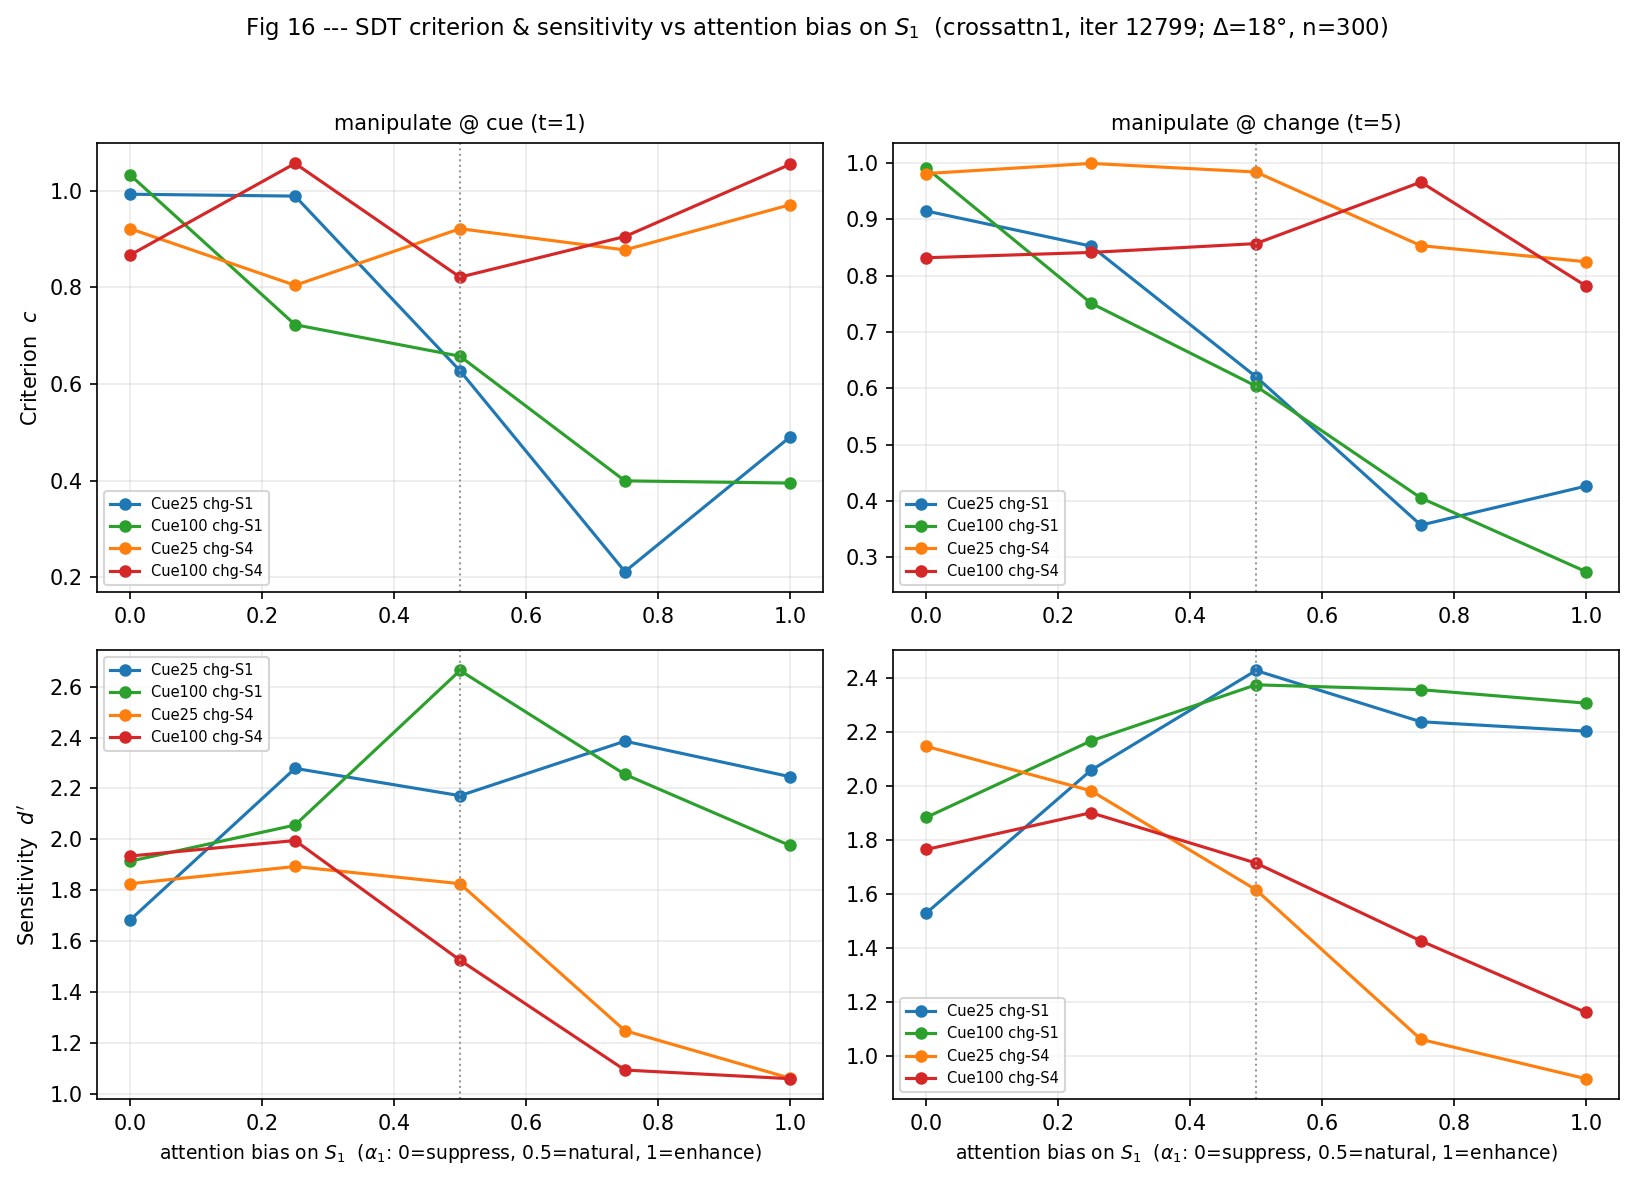
\includegraphics[width=\textwidth]{fig16_crossattn1.png}
\caption{\textbf{Fig 16 --- SDT criterion \& sensitivity vs.\ attention bias on $S_1$.} Rows: criterion
$c$, sensitivity $d'$. Columns: manipulate at cue-time ($t{=}1$) vs.\ change-time ($t{=}5$). Lines:
\{Cue $25/100\%$\}$\times$\{change at $S_1$/$S_4$\}. $\alpha_1{=}0.5$ is natural.}\label{fig:sdt16}\end{figure}

\section{Supervised vs.\ RL}
The original contrasts three training signals (supervised-actions, supervised-beliefs, RL). Our variants
are RL-only, so we faithfully reproduce the RL column across the four behavioural rows and mark the
supervised columns as out-of-scope architectural baselines that were not trained for this variant
(Fig.~\ref{fig:sup17}).

\begin{figure}[h]\centering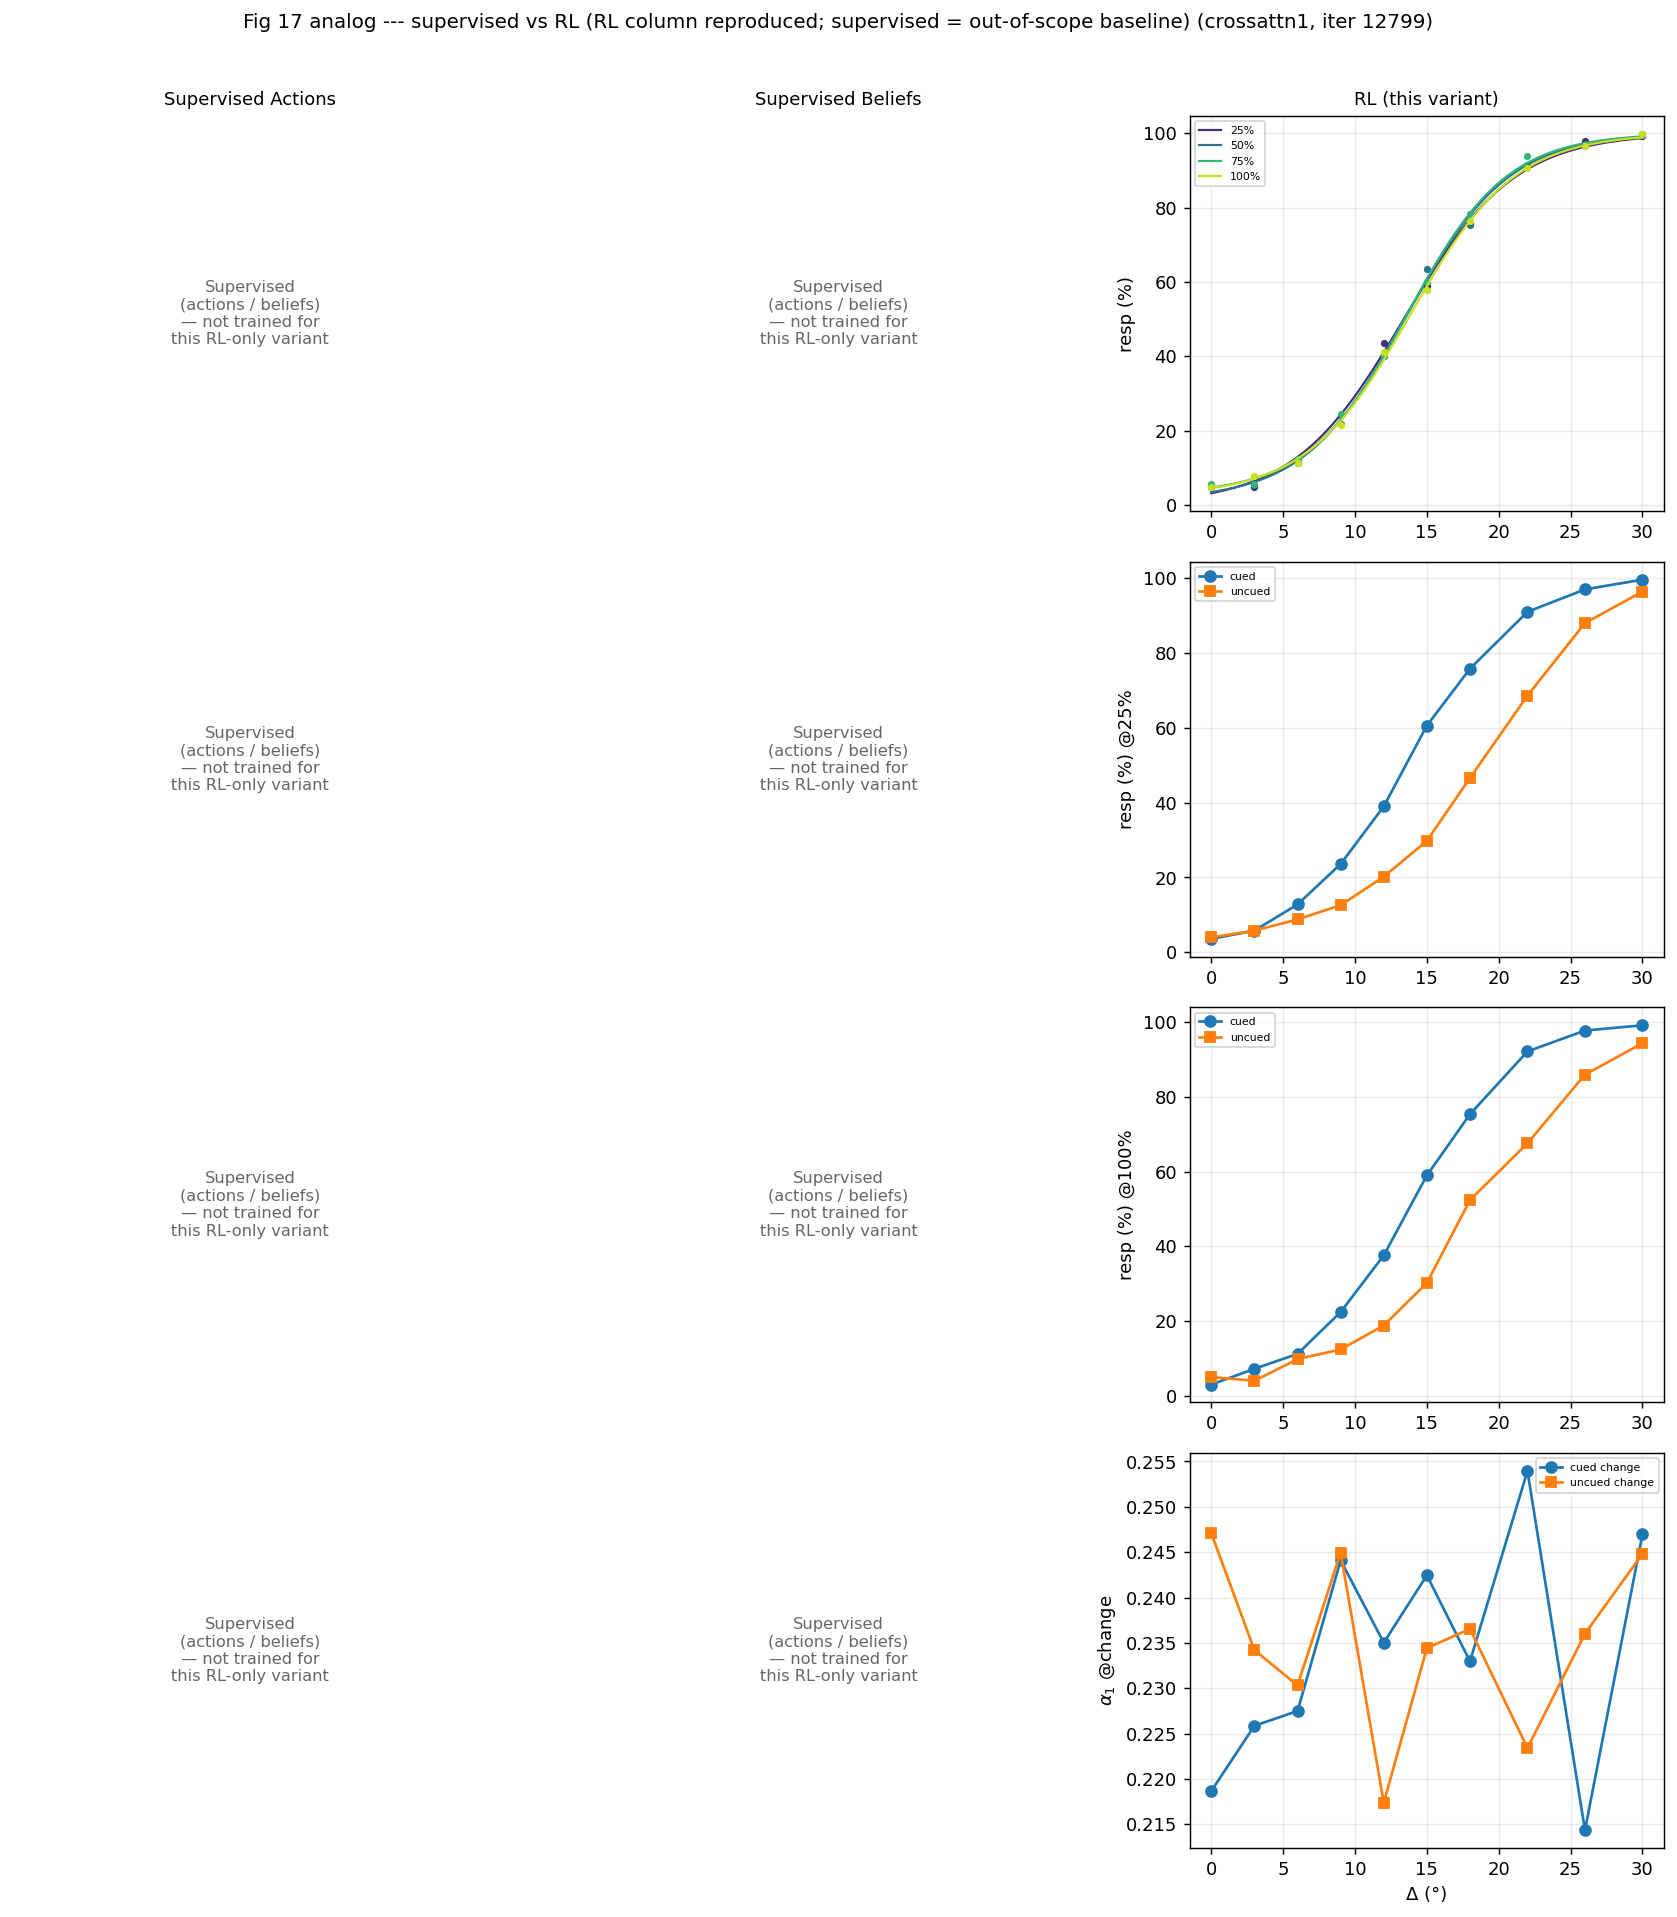
\includegraphics[width=0.9\textwidth]{fig17_crossattn1.png}
\caption{\textbf{Fig 17 analog --- supervised vs.\ RL.} RL column reproduced (response by validity;
cued vs.\ uncued at $25/100\%$; attention on $S_1$ at change vs.\ $\Delta$); supervised columns are
out-of-scope baselines for this RL-only variant.}\label{fig:sup17}\end{figure}

\section{Discussion}
The compact, pixel-trained cross-attention variant reproduces the \emph{shape} of primate-like
signatures across the whole figure set: sigmoidal psychometrics/chronometrics, a cued$>$uncued spatial
benefit, anticipatory maintenance of spatial priority, causally perturbable attention, self-attention
amplification of the change signal across memory slots, a competitive actor-logit decision axis, a
distributional value jump / TD surprise at the change, and the SDT criterion/sensitivity signatures of
attentional ``stimulation.'' It \emph{diverges} in the role of \emph{cue validity}: with a compact
memory learned from pixels, the model reads the validity ring at the cue frame but does not maintain it,
so the validity-graded modulation of the original ($d_{\mathrm{mem}}{=}1024$, VAE) does not emerge. This
dissociation---spatial cueing preserved, validity-grading lost---is itself informative about which
architectural ingredients the validity effect depends on.

\section{Methods (variant)}
\textbf{Front-end.} Each $25\times25\times3$ patch is encoded by a shared SE-ResNet to
$\hat o_i\in\mathbb R^{128}$; the token is $[\hat o_i\Vert\rho_i\Vert\tau]\in\mathbb R^{140}$.
\textbf{Cross-attention.} $Q=W_qX$, $K=[W_{kx}X\Vert W_{kh}H^{(t-1)}]$, $V=[W_{vx}X\Vert W_{vh}H^{(t-1)}]$,
$A=\mathrm{softmax}(QK^\top/\sqrt{140})$ over eight keys, $Z=X+AV$. \textbf{Memory.} A per-patch spatial
xLSTM, $d_{\mathrm{mem}}{=}128$; the flattened cell $H$ is read out. \textbf{Training.} Distributional
actor--critic on sparse reward with an auxiliary V-JEPA temporal self-distillation loss (4 heads
$\times$ 256 prototypes). \textbf{Analyses.} Behaviour uses $n{=}300$ trials/point; psychometrics fit a
4-parameter logistic $P(\Delta)=A+(1{-}A{-}B)/(1+e^{-(\Delta-D)/C})$. Attention is causally manipulated
by additively biasing the pre-softmax key scores of a location. Decoders are trained on natural states
and evaluated under modulation. SDT quantities use hit rate on change trials and false-alarm rate on
no-change trials at $\Delta{=}18^\circ$.

\end{document}
